\section{Estrutura}

Entende-se como o subsistema de estrutura as partes do sistema que possuem função estrutural. Este subsistema é responsável por comportar os demais subsistemas, seguindo os requisitos definidos pelo projeto. Para fins de melhor compreensão, os componentes da estrutura foram separados em partes, de acordo com suas características e funções.


\subsection{Compartimento de carga}

O compartimento de carga, é a caixa mais interna da estrutura, na qual o órgão, dentro das embalagens apropriadas, é transportado.

\subsubsection{Requisitos}

O compartimento de carga deve ser:

\begin{itemize}
	\item Hermeticamente fechado, ou seja, vedado;
	\item Facilmente removido ou posicionado na câmara de resfriamento.
\end{itemize}

\subsubsection{Design}

\begin{itemize}
	\item \textbf{Caixa:} De acordo com o tamanho do órgão que será carregado e as embalagens e líquido que estão envolvendo o órgão, e com os requisitos de portabilidade do sistema, o compartimento foi projetado com um design cúbico, para melhor fabricação, dimensionado para ter 24,7 x 24,7 x 20 cm.
	\item \textbf{Tampa:} O formato escolhido para a tampa da caixa foi um prato quadrado de 24,7 x 24,7 cm. Deste modo, o compartimento pode ser vedado com a aplicação de tiras de borracha nas bordas da caixa e da tampa. Uma alça posicionada no centro e topo da tampa serve para manusear o compartimento.
	\item \textbf{Fixadores:} Para que o compartimento seja hermético, a tampa deve ser bem fixada na caixa. Por isso, foram adicionados 6 presilhas distribuídas ao redor da caixa para prender a tampa.
\end{itemize}

O material escolhido para o compartimento foi aluminio, devido a sua propriedade de alta condutividade térmica, de modo a facilitar o resfriamento do interior do compartimento.

\subsubsection{Fabricação}

\underline{Materiais Utilizados:}

\begin{itemize}
	\item Chapa de alumínio série 5000 de 1m x 1m com 2 mm de espessura;
	\item Borrachas;
	\item Presilhas;
	\item Alça.
\end{itemize}

\underline{Procedimentos:}

\begin{enumerate}
	\item Inicialmente, a chapa de alumínio foi cortada utilizando cortadora de chapas.
	\item Em seguida, a chapa foi dobrada com 90° utilizando a dobradora de chapas.
	\item para finalizar a caixa foi soldada utilizando o processo TIG (tungstênio inert gás). 
	\item Foi aplicado pasta de silicone nas bordas da caixa e da tampa para ajudar na vedação. Foi fixada então a borracha utilizando cola instantânea.
	\item As presilhas foram
	\item Enfim, a alça foi posicionada no centro da tampa e rebitada para sua fixação.
\end{enumerate}

\subsubsection{Resultados}

\begin{figure}[H]
	\centering
	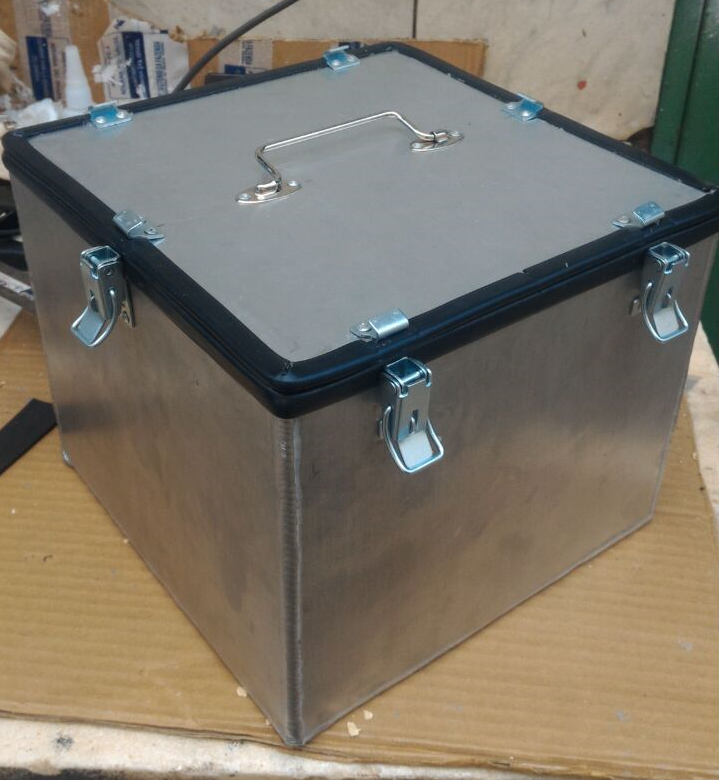
\includegraphics[scale=.4]{figuras/compartimento_de_carga.png}
	\caption{Produto final do compartimento de carga.}
\end{figure}


\subsection{Câmara de Resfriamento}

A câmara de resfriamento é a parte da estrutura resfriada pelo sistema de refrigeração e onde se encontra o compartimento de carga.

\subsubsection{Requisitos}

A estrutura da câmara de resfriamento deve ser:

\begin{itemize}
	\item Isolada termicamente;
	\item Capaz de comportar o compartimento de carga e parte interna do sistema de refrigeração;
	\item Capaz de apoiar o compartimento de carga de modo fixo, para que este não se movimente em excesso com o deslocamento da transportadora;
	\item Fixa na estrutura principal, porém seu topo deve ser acessível do lado externo.
\end{itemize}

\subsubsection{Design}

\begin{itemize}
	\item \textbf{Caixa:} Similarmente ao compartimento de carga, a câmara de resfriamento foi projetada com formato cúbico. Foram escolhidas as dimensões de 30 x 30 x 30 cm para a caixa. O material escolhido foi aço inox devido às suas excelentes propriedades de resistência e isolamento térmico.
	\item \textbf{Tampa:} A tampa da caixa é composta por uma seção quadrada de 30 x 30 cm de aço inox, uma placa de isopor de mesmas dimensões para isolamento térmico e revestimento de PVC no topo e nas laterias para proteção e acabamento. O lado interno da tampa contém apoiadores para a caixa interna.
	\item \textbf{Isolamento térmico:} Para que a câmara seja isolada termicamente, esta é cercada por uma camada de 5 cm de isopor comum em todas as faces da caixa, incluindo a tampa.
	\item \textbf{Apoios do compartimento de carga:} Para gerar melhor estabilidade para o compartimento de carga, a câmara de resfriamento possui suporte e guias para apoiar a caixa interna.
	\item \textbf{ Fixadores:} Assim como o compartimento de carga, a tampa da câmara de resfriamento é fechada por presilhas. Na câmara são utilizadas 4 presilhas, uma em cada lado do topo revestido da tampa, prendendo-a linearmente ao topo da estrutura.
\end{itemize}

\subsubsection{Fabricação}

\underline{Materiais Utilizados:}

\begin{itemize}
	\item Chapa de aço inox 304L de 1m x 2m com 1,2 mm de espessura;
	\item Placa de Isopor de 5 cm de espessura;
	\item Borrachas;
	\item Presilhas;
	\item Chapa de aço Metalon de 2 mm de espessura;
	\item Placa de PVC com 2 mm de espessura.
\end{itemize}

\underline{Procedimentos:}

\begin{enumerate}
	\item A chapa de aço foi cortada utilizando cortadora de chapas.
	\item Depois, a chapa foi dobrada em ângulos de 90° utilizando a dobradora de chapas.
	\item A solda foi realizada utilizando o processo TIG (tungstênio inert gás).
	\item Em seguida, o fundo da caixa foi amassado para tomar um formato arredondado e foi feito um furo no centro do fundo para escoamento de água.
	\item Foram cortadas e soldadas partes de chapa de aço Metalon em L para formar a base do apoiador da caixa interna, furando e rebitando no fundo da caixa. Uma placa quadrada de PVC foi posicionada na base, e tiras de PVC de aproximadamente 5 cm de largura foram fixadas nas laterais da câmara como guias para o posicionamento da caixa interna.
	\item Placas de isopor foram coladas, utilizando silicone, revestindo a caixa completamente, com excessão do topo.
	\item Foi fabricada a tampa colando uma placa de isopor em uma placa de aço inox e revestindo as laterais e o outro lado do isopor com placas de PVC. No lado de PVC da tampa, foram fixados os fechos e a alça.
\end{enumerate}

\subsubsection{Resultados}

\begin{figure}[H]
	\centering
	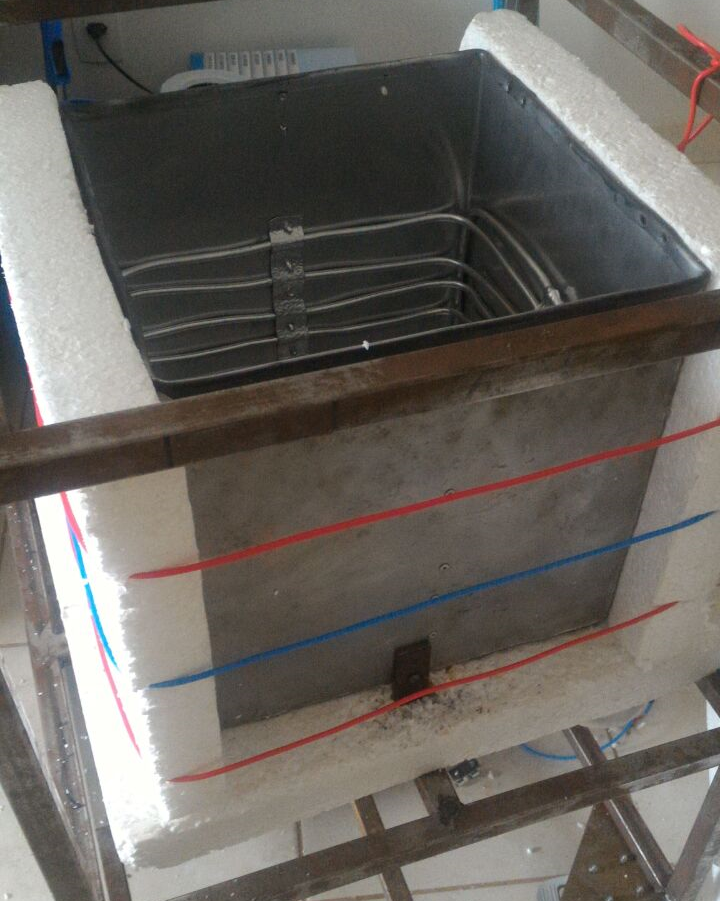
\includegraphics[height=150pt]{figuras/caixaext1.png}
	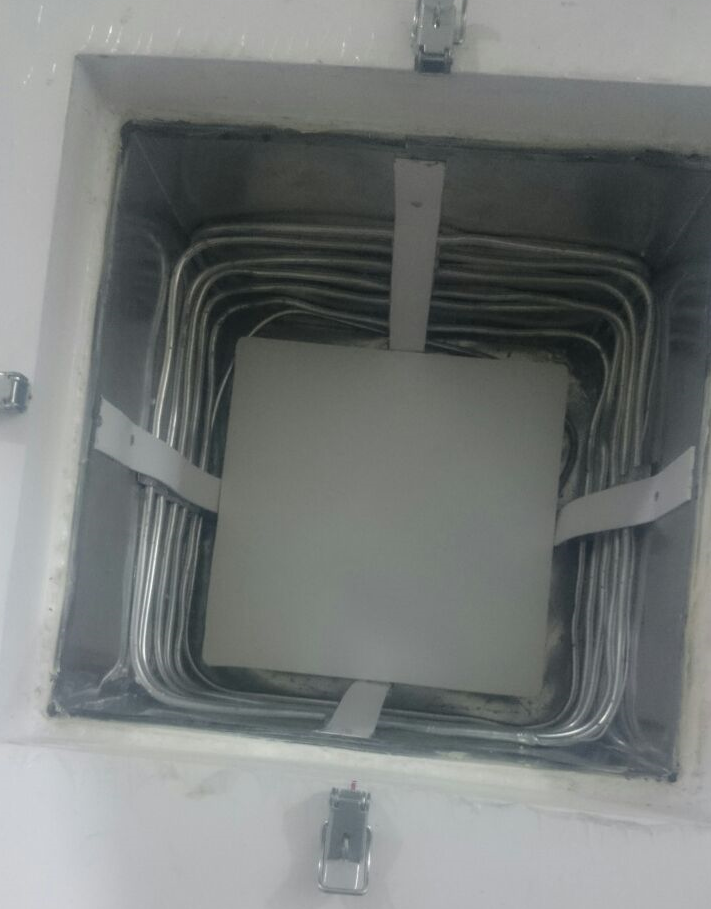
\includegraphics[height=150pt]{figuras/caixaext3.png}
	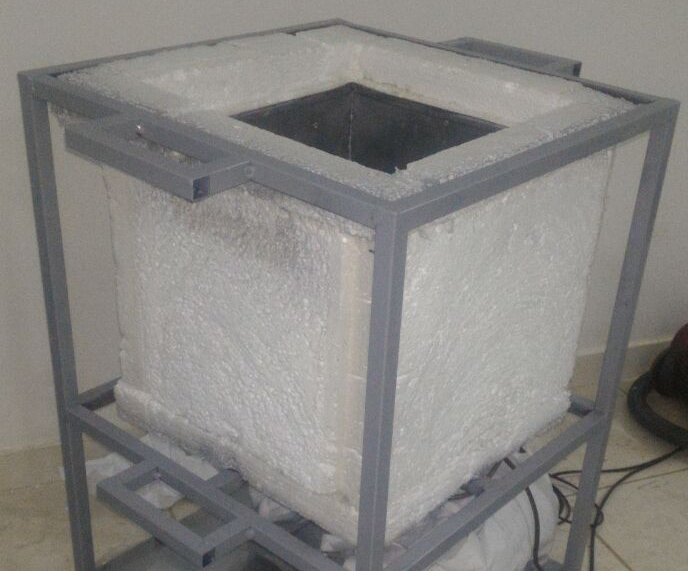
\includegraphics[height=150pt]{figuras/caixaext2.png}
	\caption{Câmara de resfriamento durante a fabricação e produto final.}
\end{figure}


\subsection{Estrutura}

Define-se aqui como estrutura a parte que de estrutura básica da transportadora, que engloba as demais partes e é responsável pela maior parte da sustentação de esforços.

\subsubsection{Requisitos}

A estrutura deve:

\begin{itemize}
	\item Ser capaz de sustentar as forças atuantes sem sofrer deformação considerável;
	\item Ter espaço interno capaz de comportar, no mínimo, a câmara de resfriamento, o sistema de refrigeração, a bateria e os subsistemas eletrônicos;
	\item Possuir apoios adequados para levantamento manual;
	\item Ser móvel.
\end{itemize}

\subsubsection{Design}

\begin{itemize}
	\item \textbf{Estrutura:} Foi projetada uma estrutura composta por barras de aço de seção quadrada de 20 x 20 mm e 1,2mm de espessura. Uma configuração de duas partes foi adotada, na qual a parte superior comporta a câmara de resfriamento e a interior comporta o compressor,  o sistema de alimentação e os sistemas eletrônicos. A estrutura também possui 4 alças, dois pares localizados em lados opostos.
	\item \textbf{Fixadores:} Para fixar a câmara de resfriamento em seu lugar na estrutura, 4 peças em formato “L” foram posicionadas de modo que um lado do fixador será preso na estrutura, e o outro lado na câmara.
	\item \textbf{Base:} Para sustentar a parte externa do sistema de refrigeração e a bateria, uma placa de alumínio será fixada no fundo da parte inferior da estrutura.
	\item \textbf{Rodas}: Para a movimentação da transportadora, o sistema tem 4 rodas, com travas, fixas embaixo da estrutura por placas triangulares soldadas nas barras inferiores.
	\item \textbf{Sistema amortecedor:} Para maior segurança do órgão, a estrutura possui um sistema de amortecimento de vibrações composto por 4 amortecedores localizados entre o final da estrutura e as rodas.
	\item \textbf{Revestimento:} Toda a estrutura é revestida por paredes de PVC, sendo uma parte dela removível para que se possa fazer manutenção dos sistemas internos.
\end{itemize}


\subsubsection{Fabricação}

\underline{Materiais Utilizados:}

\begin{itemize}
	\item Aço estrutural Metalon 20 x 20 x 1,2 mm;
	\item Chapa de aço carbono de 20 x 20 x 1,2 mm;
	\item Chapa de aço de 2 mm de espessura;
	\item Rodas
	\item Amortecedores
	\item 
	\item Chapa de PVC de espessura 2 mm.
\end{itemize}

\underline{Procedimentos:}

\begin{enumerate}
	\item As barras foram cortadas com a esmerilhadora utilizando um disco próprio para corte do metal. Após cortadas foram corrigidas e acabadas com um esmeril fixo.
	\item A solda foi realizada utilizando o processo MIG (metal inert gás) e desbastadas com a máquina esmerilhadora utilizando o disco esmerilhador.
	\item Os fixadores da caixa de refrigeração foram soldados na estrutura com um ângulo de 90 graus e esmerilhados para o acabamento da solda.
	\item As placas de aço carbono de fixação do sistema compressor e da barteria foram fixadas com rebites nos buracos feitos na estrutura com uma furadeira.
	\item Barras de metalon foram cortadas e soldadas para formar as 4 alças da estrutura. Estas alças foram soldadas nas barras superiores e do meio da estrura em 2 lados opostos.
	\item Na parte inferior da estrutura foram soldadas placas triangulares de aço nos cantos, nas quais os amortecedores foram presos.
	\item Barras de aço metalon foram cortadas e soldadas formando um quadrado e depois foram feitas 4 peças em formato L do mesmo material, as quais foram soldadas nos cantos do quadrado.
	\item O lado livre dos amortecedores foi parafusado nos cantos do quadrado, de modo que estes ficaram entre a parte inferior da estrutura e o quadrado. As rodas foram presas, com parafusos, nas peças em L soldadas no quadrado.
	\item As placas de PVC foram cortadas e rebitadas na estrutura cercando-a completamente, com exceção de uma secção quadrada cujo tamanho é a metade de um dos lados. Esta secção é presa à estrutra por velcro, de modo que pode ser facilmente removida para que o interior da transportadora seja acessado, na parte que contém o sistema de alimentação e sistemas eletrônicos.
\end{enumerate}

\subsubsection{Resultados}

\begin{figure}[H]
	\centering
	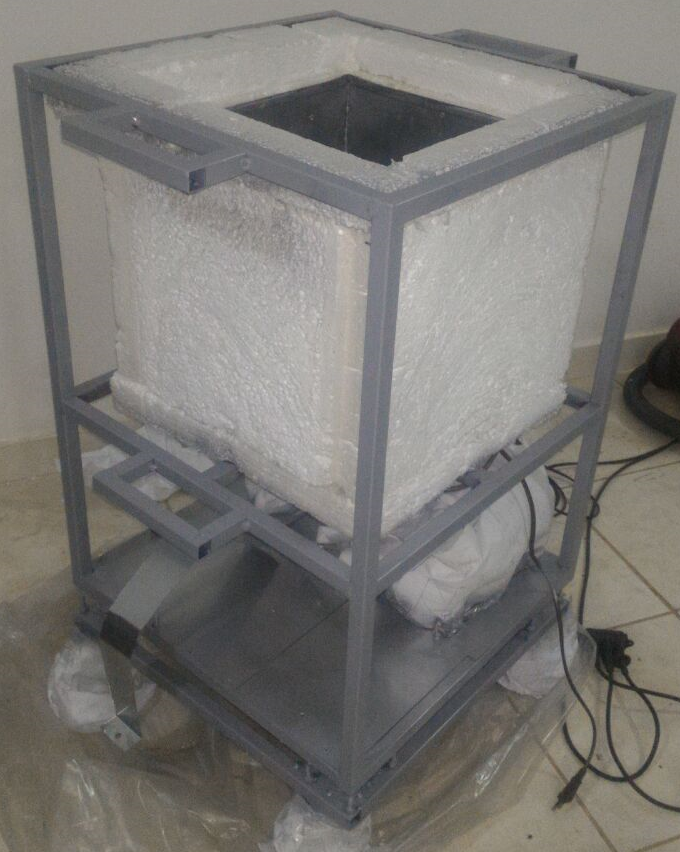
\includegraphics[width=250pt]{figuras/estrutura_fab.png}
	\caption{Estrutura principal sem o revestimento}
\end{figure}

\begin{figure}[H]
	\centering
	\includegraphics[width=250pt]{figuras/amortecimento.png}
	\caption{Sistema de amortecimento}
\end{figure}

\begin{figure}[H]
	\centering
	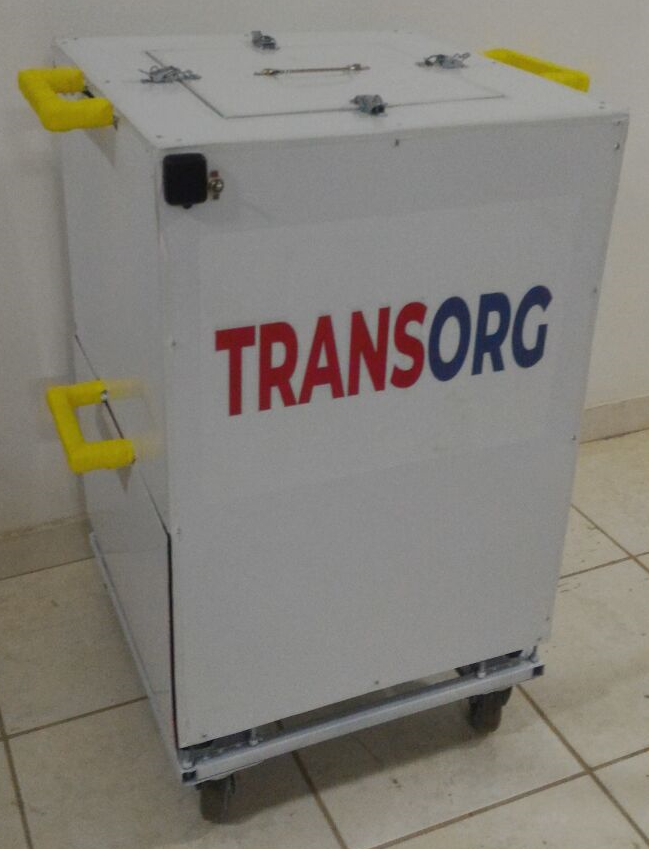
\includegraphics[width=250pt]{figuras/estrutura_final.png}
	\caption{Produto final da estrutura}
\end{figure}

\subsection{Sistema de amortecimento}

\subsubsection{Análise computacional de vibrações da estrutura}

\noindent Importação do modelo para o software Ansys:

\begin{enumerate}
	\item Aplicando material em cada componente
	\begin{itemize}
		\item Estrutura: aço estrutural
		\item Câmara interna: alumínio
		\item Câmara externa: aço inoxidável
	\end{itemize}
	\item Aplicação das conexões no modelo sem amortecimento
	\begin{itemize}
		\item Estrutura e Câmara Externa: joint fixa
		\item Câmara Interna e Externa: joint fixa
		\item Base da estrutura e solo: joint fixa
	\end{itemize}
	
	\begin{figure}[H]
		\centering
		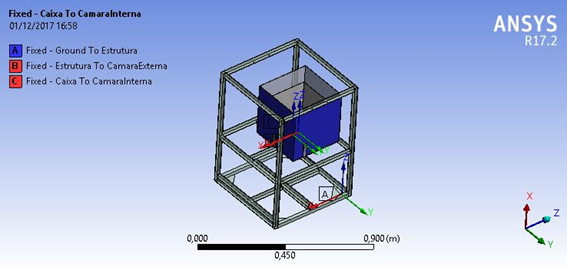
\includegraphics[width=350pt]{figuras/conexoes_sem_amortecimento.png}
		\caption{Conexões no modelo sem amortecimento.}
	\end{figure}
	
	\item Aplicação das conexões no modelo com amortecimento
	\begin{itemize}
		\item Estrutura e Câmara Externa: joint fixa
		\item Câmara Interna e Externa: joint fixa
		\item Base da estrutura e solo: joint fixa
		\item Base da estrutura e estrutura: spring
	\end{itemize} 
	
	\begin{figure}[H]
		\centering
		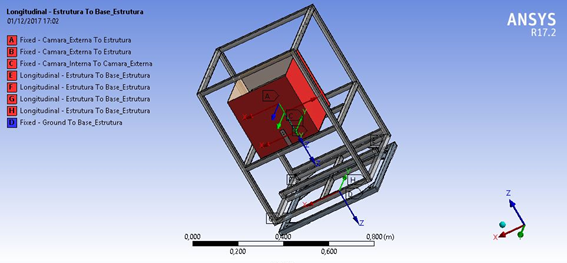
\includegraphics[width=350pt]{figuras/conexoes_com_amortecimento.png}
		\caption{Conexões no modelo com amortecimento.}
	\end{figure}
	
	\item Criação da malha
	
	\begin{figure}[H]
		\centering
		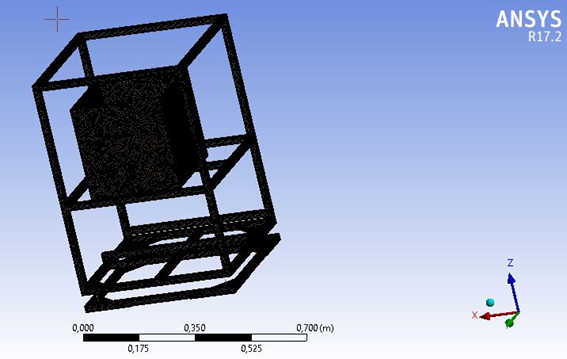
\includegraphics[width=350pt]{figuras/malha.png}
		\caption{Malha do utilizada no modelo.}
	\end{figure}
	
	\item Analise modal sem amortecimento
	
	\begin{itemize}
		\item Deslocamento restrito à vertical
		
		\begin{figure}[H]
			\centering
			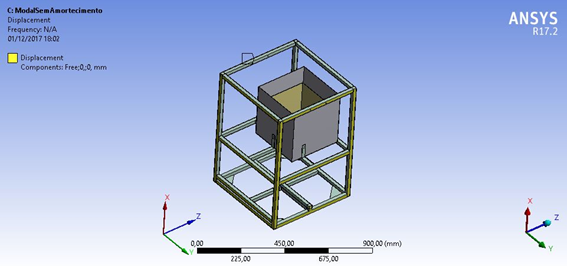
\includegraphics[width=350pt]{figuras/restricao1.png}
			\caption{Restrição de deslocamento para modelo sem amortecimento.}
		\end{figure}
		
		\item Como solução foi obtido os dez primeiros modos de vibração assim como suas frequências naturais.
	\end{itemize}
	
	\begin{table}[H]
		\centering
		\caption{Resultados para os seis primeiros modos de vibração.}
		\begin{tabular}{|l|l|l|}
			\hline
			Modo de vibração & Frequência {[}Hz{]} & Deslocamento {[}mm{]} \\ \hline
			1º               & 236,38              & 768,43                \\ \hline
			2º               & 246,25              & 683,05                \\ \hline
			3º               & 335,82              & 597,67                \\ \hline
			4º               & 568,46              & 512,29                \\ \hline
			5º               & 572,86              & 426,91                \\ \hline
			6º               & 600,57              & 341,53                \\ \hline
		\end{tabular}
	\end{table}
	
	\begin{figure}[H]
		\centering
		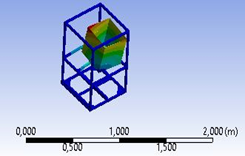
\includegraphics[height=130pt]{modo1_1.png}
		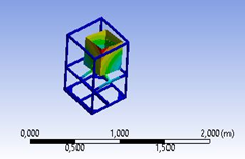
\includegraphics[height=130pt]{modo1_2.png}
		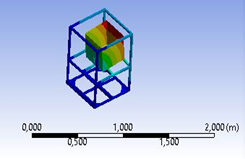
\includegraphics[height=130pt]{modo1_3.png}
		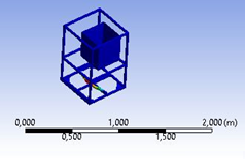
\includegraphics[height=130pt]{modo1_4.png}
		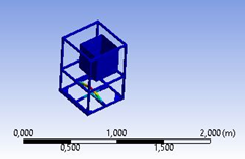
\includegraphics[height=130pt]{modo1_5.png}
		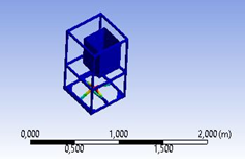
\includegraphics[height=130pt]{modo1_6.png}
		\caption{6 primeiros modos de vibração.}
	\end{figure}
	
	\item Analise modal com amortecimento
	
	Para considerar o amortecimento foram obtidos de cálculos analíticos a constante de amortecimento e a constante de mola para o coxim de borracha natural.
	
	Constante de amortecimento = 2239,04 [N.s/m]
	
	Constante de mola = 73080 [N/m]
	
	\begin{itemize}
		\item Deslocamento restrito a vertical
		
		\begin{figure}[H]
			\centering
			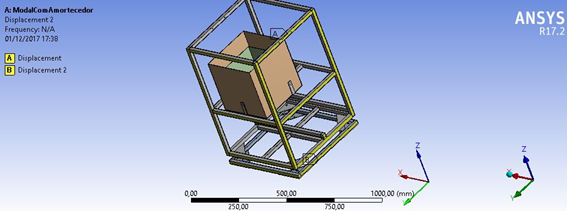
\includegraphics[width=350pt]{figuras/restricao2.png}
			\caption{Restrição de deslocamento para modelo com amortecimento.}
		\end{figure}
		
		\item Como solução, foi obtido os dez primeiros modos de vibração assim como suas frequências naturais.
	\end{itemize}
\end{enumerate}

\begin{table}[H]
	\centering
	\caption{Resultados utilizando o modelo com amortecimento.}
	\begin{tabular}{|l|l|l|}
		\hline
		Modo de vibração & Frequências {[}Hz{]} & Deslocamento máximo {[}mm{]} \\ \hline
		1º Modo          & 20,621               & 7,66                         \\ \hline
		2º Modo          & 207,86               & 22,6                         \\ \hline
		3º Modo          & 221,98               & 22,7                         \\ \hline
		4º Modo          & 396,37               & 15,49                        \\ \hline
		5º Modo          & 560,99               & 85,03                        \\ \hline
		6º Modo          & 572,98               & 78,83                        \\ \hline
	\end{tabular}
\end{table}

\begin{figure}[H]
	\centering
	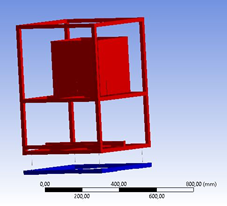
\includegraphics[height=130pt]{figuras/modo2_1.png}
	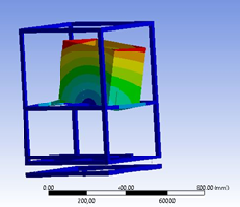
\includegraphics[height=130pt]{figuras/modo2_2.png}
	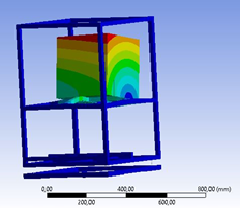
\includegraphics[height=130pt]{figuras/modo2_3.png}
	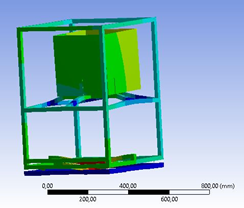
\includegraphics[height=130pt]{figuras/modo2_4.png}
	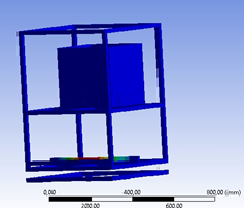
\includegraphics[height=130pt]{figuras/modo2_5.png}
	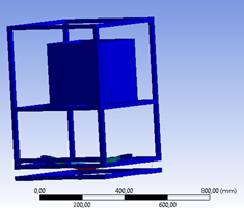
\includegraphics[height=130pt]{figuras/modo2_6.png}
	\caption{6 primeiros modos de vibração com amortecimento.}
\end{figure}

Assim, concluímos que o sistema de amortecimento proposto para o projeto é satisfatório, pois os valores de deslocamento com o sistema de amortecimento foram mais baixos que os valores de deslocamento para o sistema sem amortecimento.

\subsubsection{Dimensionamento do coxim}

Quando se fala em componentes de amortecimento a dureza é um importante parâmetro a ser levado em conta no dimensionamento decomponentes. Existem várias escalas utilizadas para definir o grau de dureza de uma borracha. Aqui utilizaremos a escala Shore A, que é mais utilizada em borrachas macias.

\begin{figure}[H]
	\centering
	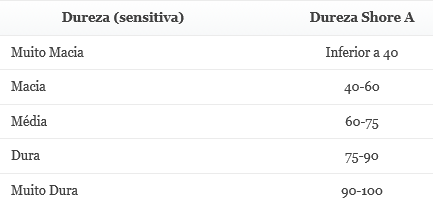
\includegraphics[width=300pt]{figuras/tabela_dureza.png}
	\caption{Classe de dureza de acordo com a maciez da borracha.}
\end{figure}

\underline{Informações iniciais:}

\begin{itemize}
	\item Dureza = 55 Shore A. Ec = 30,5 kgf / cm²  = 2,991 MPa;
	\item Diâmetro = 2,3 cm;
	\item Comprimento = 3,4 cm;
	\item Quantidade de coxins = 4;
	\item Massa suspensa = +- 50 kg;
	\item Deflexão = 1,4 mm/70 kg.
\end{itemize}

\begin{figure}[H]
	\centering
	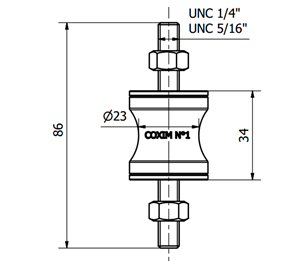
\includegraphics[width=200pt]{figuras/dimensoes_coxim.png}
	\caption{Coxim escolhido para o projeto.}
\end{figure}

\begin{itemize}
	\item \underline{Dimensionamento estático:}
\end{itemize}

\noindent Fator de forma: 

\noindent Ff = As/Al = adimensional

\noindent As = área superficial solicitada por um ou mais forças cm²

\noindent Al = somatória das áreas livres da mola = cm²

\begin{figure}[H]
	\centering
	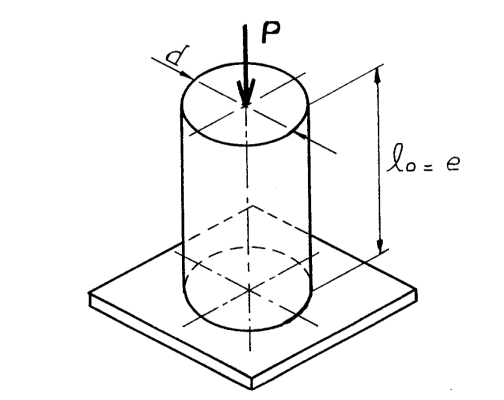
\includegraphics[width=200pt]{forma_cilindro.png}
	\caption{Forma geométrica cilíndrica.}
\end{figure}

\[F_f = \frac{d}{4 \cdot l_0} = \frac{2,3}{4 \cdot 3,4} = 0,17\]


\noindent Procedimento para determinação do coeficiente de rigidez do coxim selecionado:

\noindent Solicitação por compressão (carga máxima em cada coxim):

\begin{figure}[H]
	\centering
	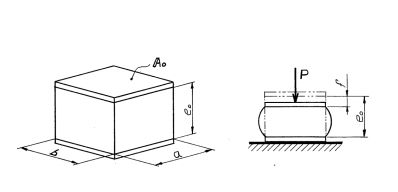
\includegraphics[width=250pt]{figuras/compressao.png}
	\caption{Solicitação da mola por compressão.}
\end{figure}

\noindent Área de sessão transversal da borracha:


\[A_0= \pi \frac{d^2}{4}= \pi \frac{2,3^2}{4} = 4,15 \ cm^2\]


\noindent Tensão por compressão (carga máxima suportada):

\[{\sigma}_c = \frac{P}{A_0} = \frac{70}{4,15} = 16,87 \ \frac{kgf}{cm^2}\]

\noindent Encruamento devido a solicitação da carga:

\[f = \frac{P.e_0}{A_0.E_c} = \frac{70.3,4}{4,15.30,5} = 1,88 \ cm\] 

\noindent Deformação devido a solicitação da carga:

\[{\epsilon }_c=\frac{f}{e_0}=\frac{0,94}{3,4}=0,55\] 

\noindent Coeficiente de rigidez:

\[K = E_c\frac{A_0}{e_0} = \frac{30,5 \cdot 4,15}{3,4} = 37,23 \ \frac{kgf}{cm} = 36,5 \ \frac{kN}{m} \]

\begin{itemize}
	\item \underline{Dimensionamento dinâmico:}
\end{itemize}

\noindent Frequência oscilatória natural:

\[f_n = \frac{1}{T_n} = \frac{1}{2 \pi \cdot \sqrt{\frac{m}{k}}} = \frac{1}{2\pi}\sqrt{\frac{k}{m}} \ \left[Hz\right]\ \]

\[m = massa = \frac{P}{g} \left[utm\right]\] 

\[g = acelera\textrm{\c{c}}\textrm{\~{a}}o\ da\ gravidade=981\left[\frac{cm}{s^2}\right]\] 

\[T_n=per\textrm{\'{i}}odo\ de\ um\ ciclo\ completo\ da\ frequ\textrm{\^{e}}ncia\ natural=[s]\] 

\[f_n=\frac{1}{2.\pi }.\sqrt{\frac{70,40}{\frac{70}{981}}}=5\ \left[Hz\right]\] 

\[T_n=\frac{1}{f_n}=\frac{1}{5}=0,2\ [s]\] 

\noindent Ressonância corre quando:

\[\frac{f_e}{fn}=1\] 

\[f_e=frequ\textrm{\^{e}}ncia\ de\ excita\textrm{\c{c}}\textrm{\~{a}}o=\left[Hz\right]\] 

\begin{figure}[H]
	\centering
	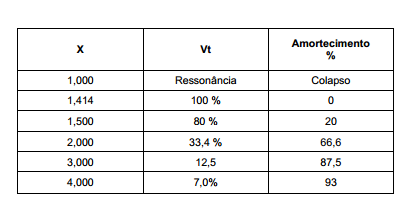
\includegraphics[width=250pt]{figuras/vibracao_transmitida.png}
	\caption{Vibração transmitida em função da razão de vibração.}
\end{figure}

O correto dimensionamento de componentes da suspensão parte do estudo dinâmico de seus componentes. O principal parâmetro a ser dimensionado é o coeficiente de amortecimento do amortecedor. Para o estudo consideraremos o modelo de 1/4 de veículo, como mostra a figura \ref{modelomassa}.

\begin{figure}[H]
	\centering
	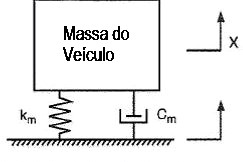
\includegraphics[width=150pt]{figuras/sistema_massa.png}
	\caption{Modelo de 1/4 de veículo.}
	\label{modelomassa}
\end{figure}

A partir deste modelo podemos retirar a equação de movimento do sistema:

\begin{equation} \label{mov2}
m\ddot{x}+ C \dot{x} + kx = 0 
\end{equation} 

\begin{equation} \label{mov3} 
C=2\xi w_N 
\end{equation} 

\begin{equation} \label{mov4} 
k = {w_N}^2 
\end{equation} 

Podemos reescrever a equação \eqref{mov2} como:

\begin{equation} \label{mov5} 
m\ddot{x} + 2\xi w_N\dot{x} + w^2_Nx = 0
\end{equation} 

A solução para o caso sub-amortecido é:

\begin{equation} \label{mov6} 
x=x_0e^{-\xi w_Nt}sen\left(w_Dt + \Phi \right) 
\end{equation} 

A solução para o caso não amortecido:

\begin{equation} \label{mov7} 
x = x_0sen(w_Nt + \Phi)
\end{equation} 

Sabemos que:

\begin{equation} \label{mov8} 
w_D = w_N\sqrt{1 - {\xi }^2}
\end{equation} 

Onde: 

\noindent $w_D$ = frequência natural amortecida

\noindent $w_N$ = frequência natural não amortecida

\noindent $\xi$ = fator de amortecimento

A frequência natural não amortecida é obtida através da seguinte equação:

\begin{equation} \label{mov9}
w_N = \sqrt{\frac{k}{m}}
\end{equation} 

Onde:

\noindent K = constante elástica da mola $\left[\frac{N}{m}\right]\ $

\noindent m = massa amortecida [kg]

O fator de amortecimento ($\xi$) caracteriza a resposta da massa suspensa no tempo durante uma perturbação e pode ser representada matematicamente como a relação entre o coeficiente de amortecimento (C) e o coeficiente de amortecimento crítico ($C_{crit}$).

\begin{equation} \label{mov10}
\xi =\frac{c}{c_{crit}}=\frac{c}{\sqrt{2km}} 
\end{equation} 

Com base nas informações acima podemos calcular o coeficiente de amortecimento para o amortecedor adequado ao projeto.

Escolhendo o fator de amortecimento de 0,7 pelo fato dele proporcionar uma única oscilação antes da estabilização, a massa de 70 kg e a constante elástica da mola de 73,08 kN/m, podemos calcular o coeficiente de amortecimento para o amortecedor a partir da equação \eqref{mov10}:

\[c = \xi \sqrt{2km} = 0,7 \cdot \sqrt{2 \cdot 73080 \cdot 70} = 2239,04 \ \left[ \frac{Ns}{m} \right] \]

\begin{figure}[H]
	\centering
	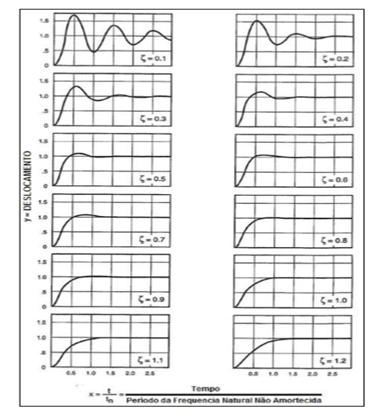
\includegraphics[width=250pt]{figuras/deslocamento_amortecido.png}
	\caption{Resposta do sistema para alguns fatores de amortecimentos.}
\end{figure}

\subsubsection{Teste e validação do sistema}

Após a fabricação e integração da estrutura, foram realizados dois testes para obter as frequências de vibração no interior da caixa na qual o órgão é transportado. O teste foi feito empurrando a estrutura por 3 m em dois tipos de piso, um piso externo de cimento e um piso interno semelhante a piso hospitalar. O primeiro teste foi feito sem o sistema de amortecimento e o segundo com o sistema. Os resultados foram obtidos por um aplicativo para celular Android chamado VibSensor, o qual utiliza o acelerômetro embutido do aparelho para obter dados de aceleração em três eixos de coordenadas. Os resultados, em gráfico para os testes foram:


\begin{figure}[H]
	\centering
	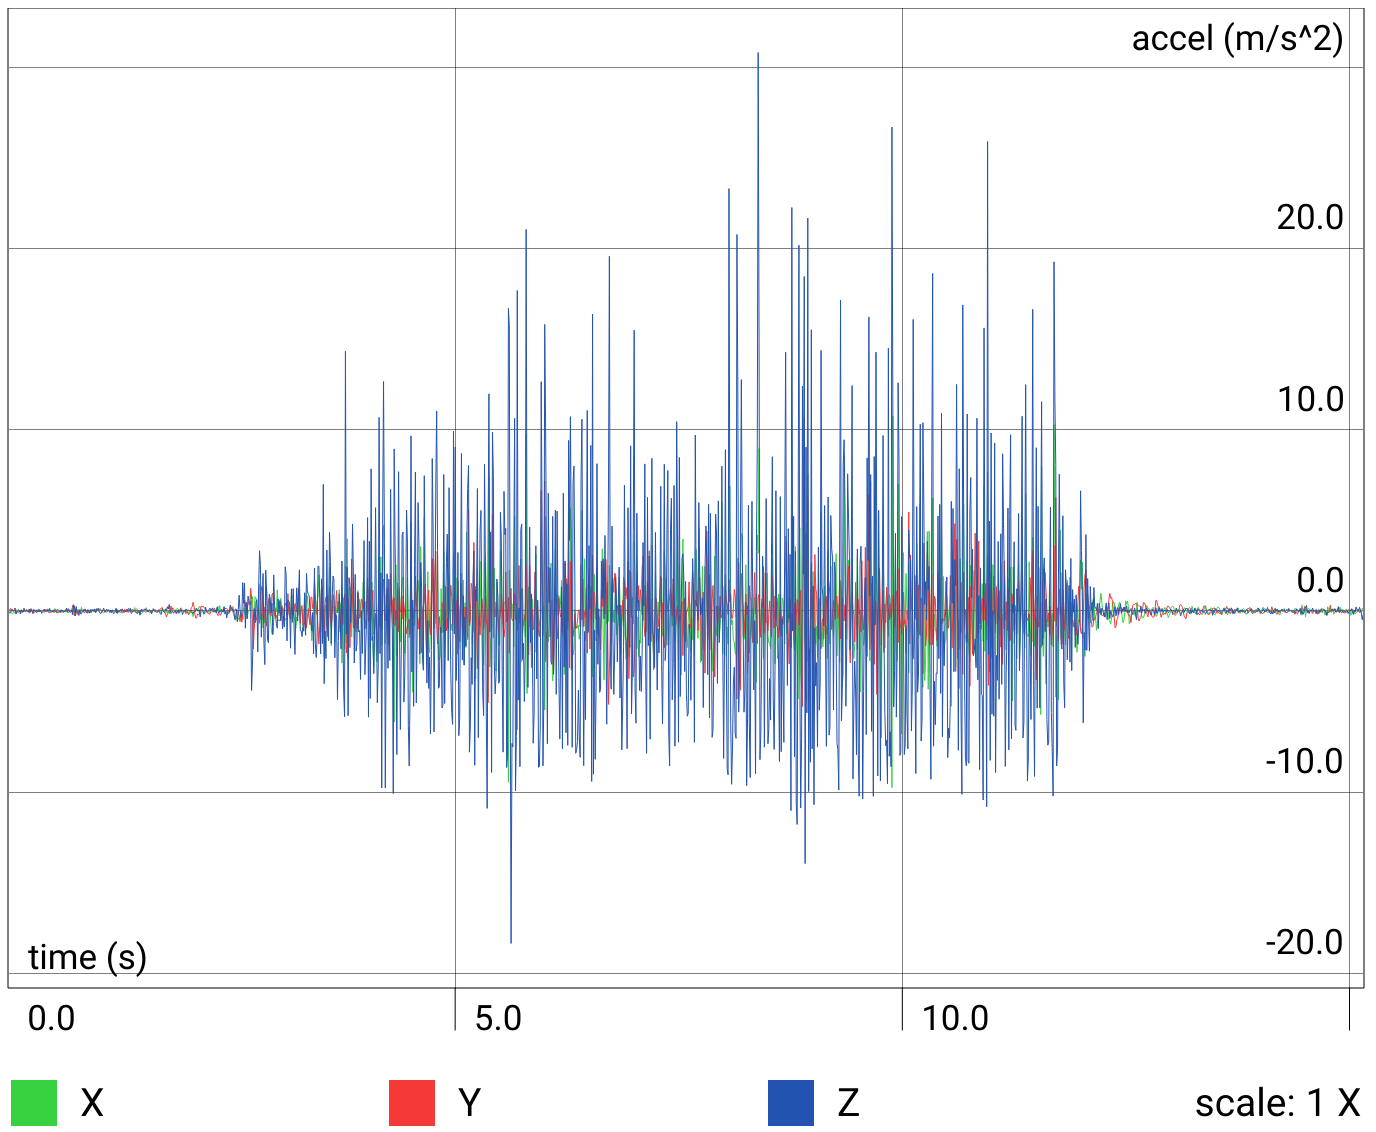
\includegraphics[height=190pt]{figuras/piso_ext_sem_amortecimento.png}
	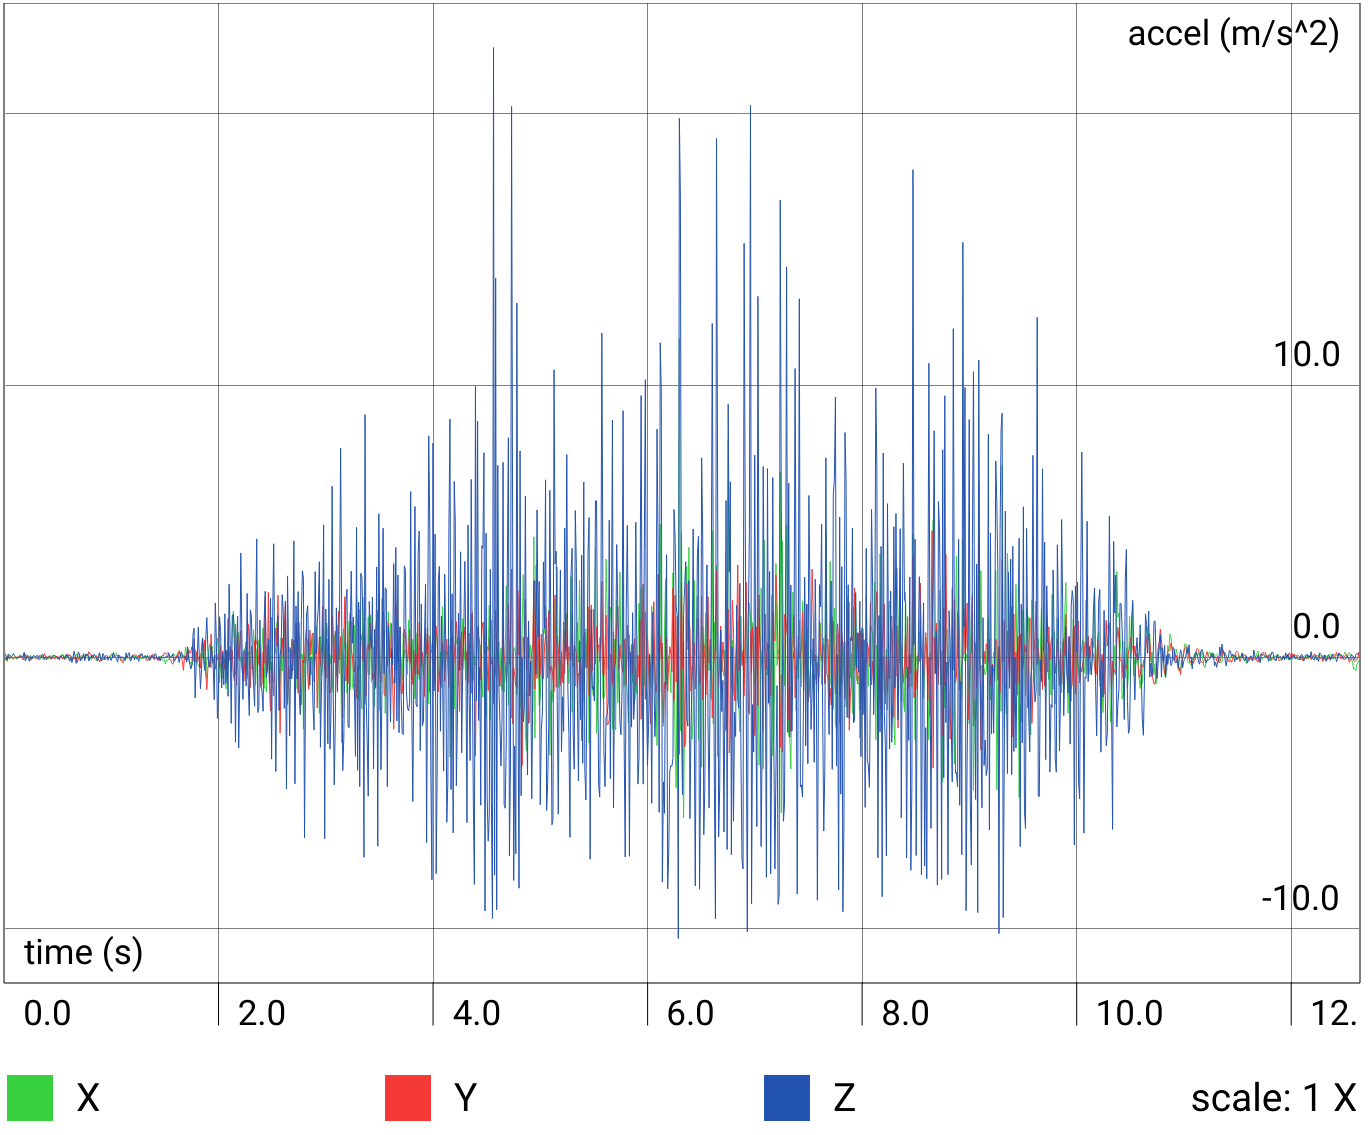
\includegraphics[height=190pt]{figuras/piso_ext_com_amortecimento.png}
	\caption{Resultado de aceleração antes e depois da aplicação do amortecimento para teste em piso externo.}
\end{figure}

\begin{figure}[H]
	\centering
	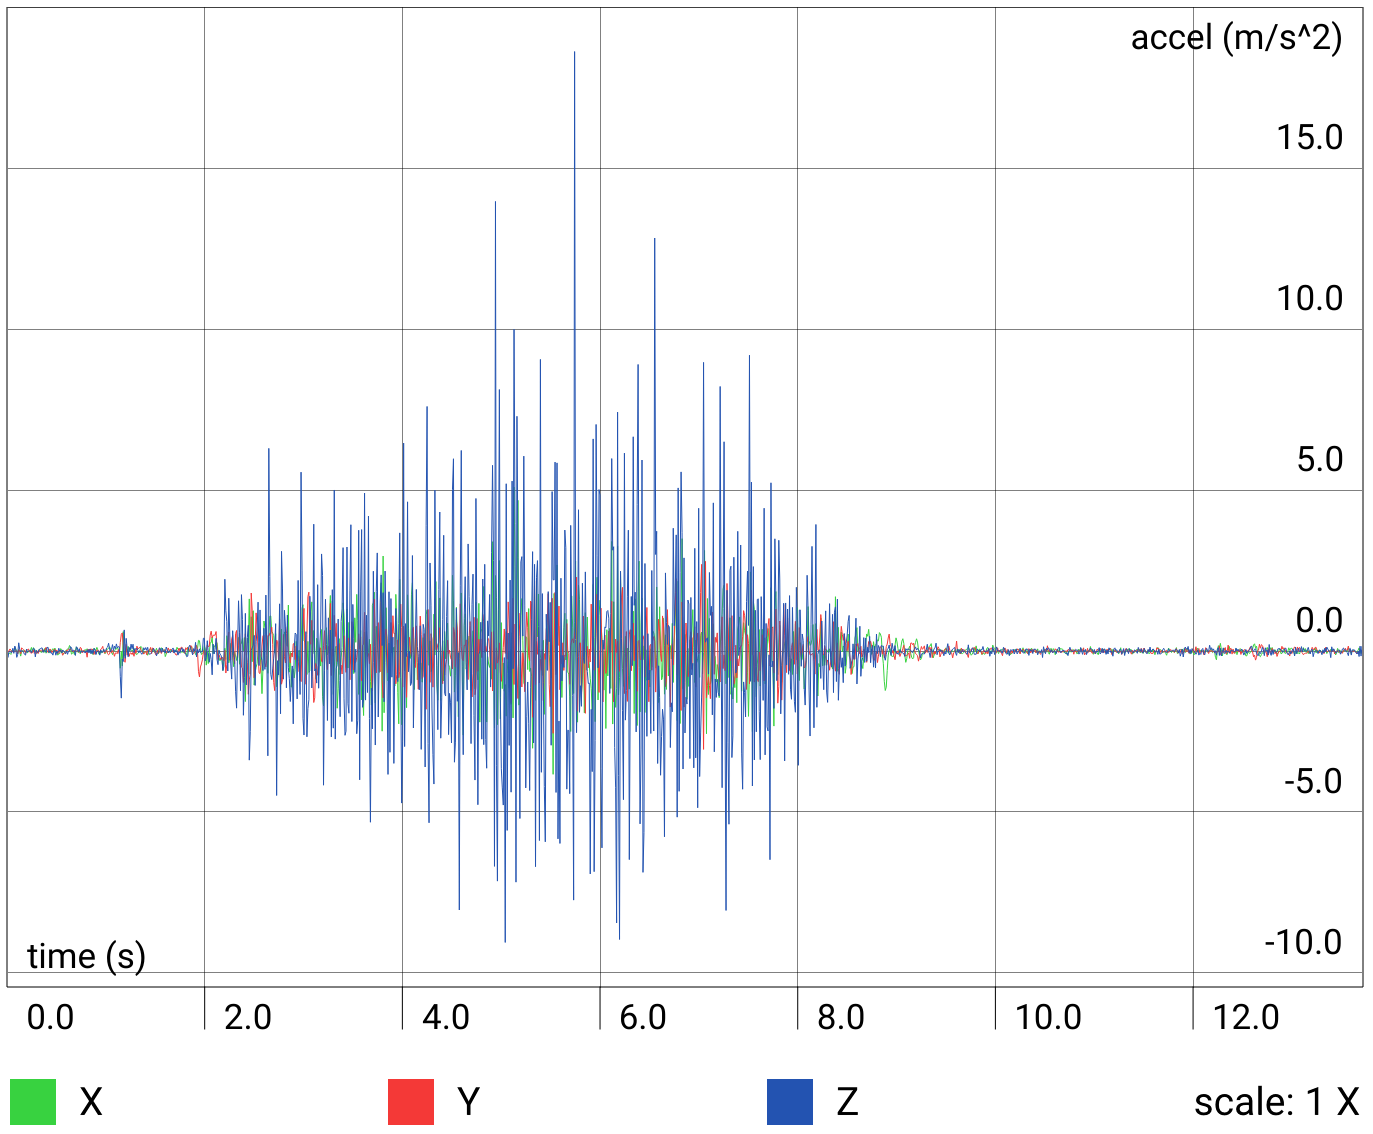
\includegraphics[height=190pt]{figuras/piso_int_sem_amortecimento.png}
	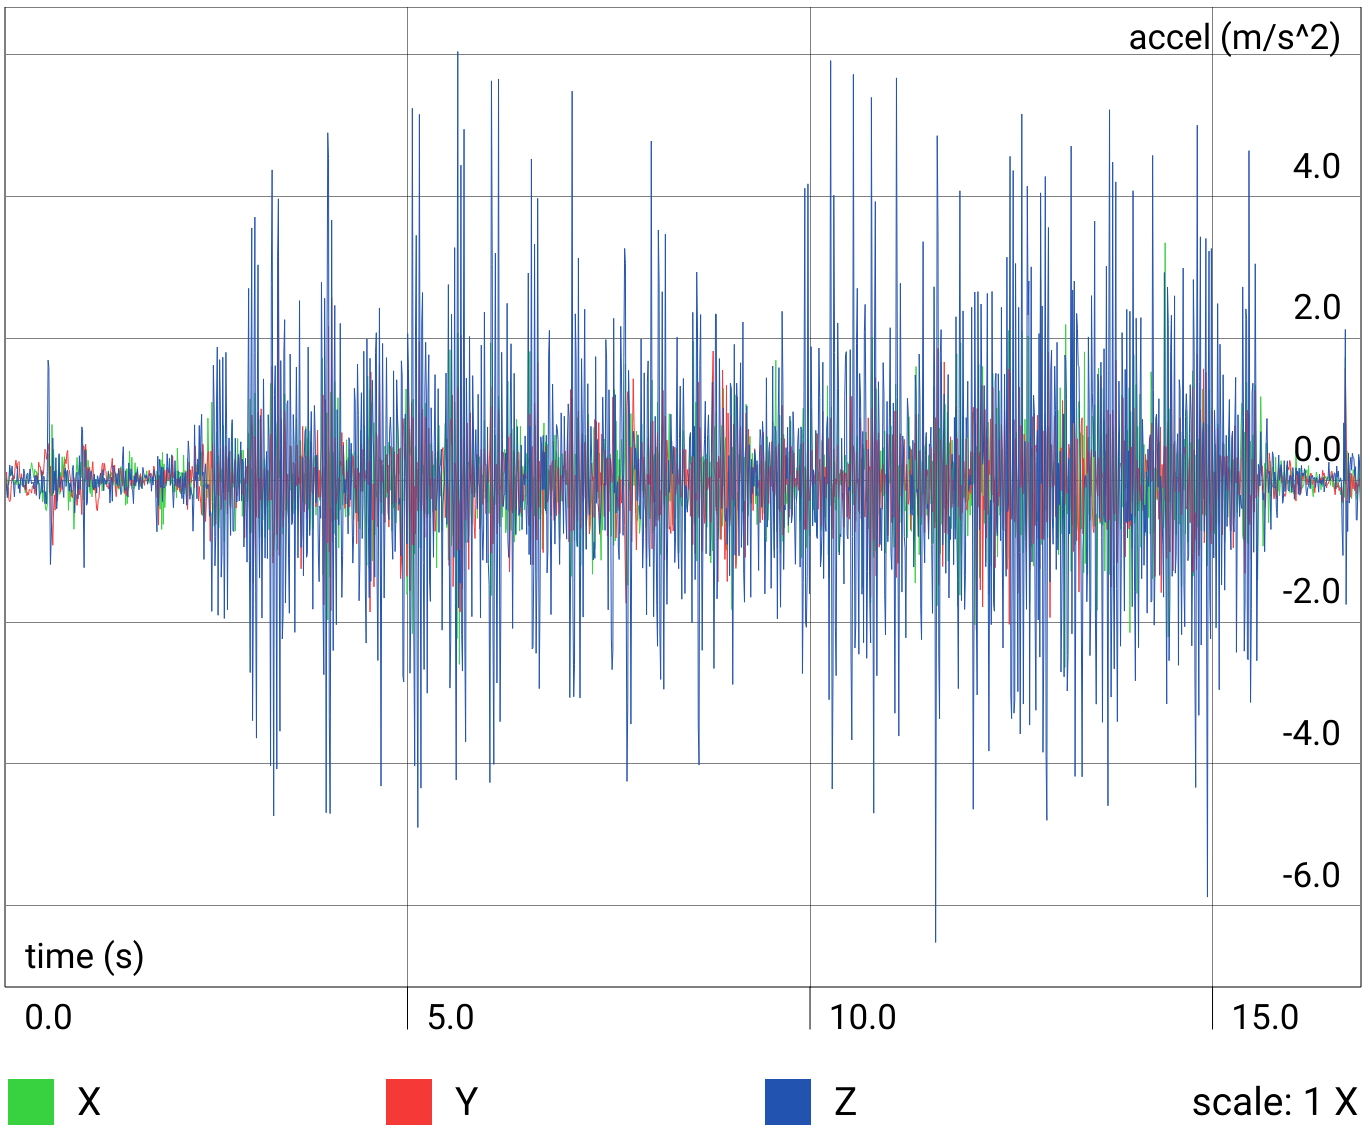
\includegraphics[height=190pt]{figuras/piso_int_com_amortecimento.png}
	\caption{Resultado de aceleração antes e depois da aplicação do amortecimento para teste em piso interno.}
\end{figure}

\begin{table}[H]
	\centering
	\caption{Resultados de vibração obtidos no teste}
	\label{vibteste}
	\begin{tabular}{|c|c|c|}
		\hline
		\textbf{Configuração do Teste}    & \textbf{Maior aceleração obtida [$^2$]} & \textbf{Frequência [Hz]} \\ \hline
		Em piso externo   & 30        & 10,47           \\
		sem amortecimento &                    &            \\ \hline
		Em piso externo   & 22        & 9,927           \\
		com amortecimento &                    &            \\ \hline
		Em piso interno   & 18        & 12,39           \\ 
		sem amortecimento &                    &            \\ \hline
		Em piso interno   & 6         & 8,195           \\
		com amortecimento &                    &            \\ \hline
	\end{tabular}
\end{table}

Observando os valores de aceleração, é notável a diminuição destes após a aplicação de amortecimento na estrutura, o que valida o seu funcionamento. E as frequências medidas foram todas consideravelmente menores que as frequências de ressonância da estrutura obtidas na análise computacional, o que indica uma grande improbabilidade de falha por vibração.

\subsection{Simulação Computacional}

\subsubsection{Análise Estrutural}

O Método dos Elementos dos Elementos Finitos (MEF) é considerado como um método matemático capaz de resolver problemas complexos de forma eficiente e rápida. Lotti (2006), define o MEF como sendo um modelo matemático em meio contínuo que é discretizada em elementos, mantendo as propriedades do objeto em análise. Qualquer falha em componentes estruturais é iniciada após a tensão aplicada exceder o limite de escoamento do material naquele local, Beer e Johnston (1982). Com base nisso utilizaremos o MEF para analisar a viabilidade estrutural do projeto.

Para análise estática cada elemento utilizado na geração da malha é interpretado como uma mola com uma dada rigidez e tamanho determinado. Esta consideração faz com que possamos construir matrizes em termos de carregamento, deslocamentos e rigidez, onde a rigidez depende das propriedades dos materiais e da geometria da peça em análise.

\paragraph*{Condições de Contorno}\

\begin{table}[H]
	\centering
	\caption{Condições de Contorno da Análise Estrutural}
	\label{condcontornoestrut}
	\begin{tabular}{|c|c|c|}
		\hline
		Peça                   & Restrição                            & Carregamento {[}N{]}\\ \hline
		Estrutura              & Engaste na extremidade inferior      & 120+120  \\ \hline
		Compartimento de Carga & Contato fixo nos apoios              & 100 \\ 
		& da câmara de resfriamento            &     \\ \hline
		Câmara de Resfriamento & Contato fixo nos apoios da estrutura & --  \\ \hline
	\end{tabular}
\end{table}

\paragraph*{Resultados}\

\begin{figure}[H]
	\centering
	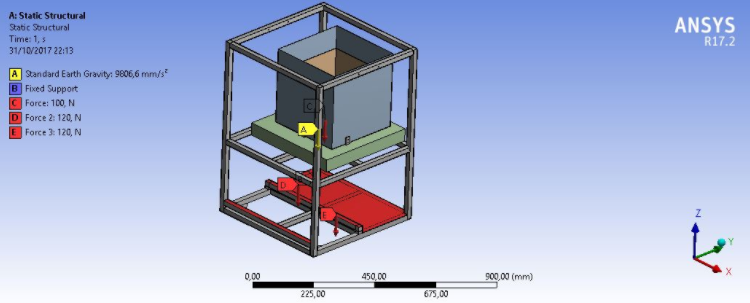
\includegraphics[]{figuras/carregamentos.png}
	\caption{Carregamentos}
\end{figure}

\begin{figure}[H]
	\centering
	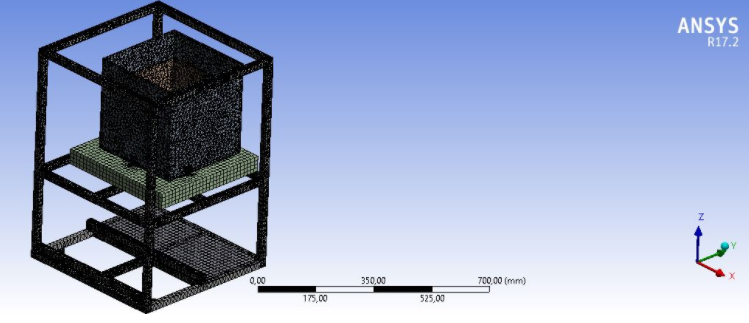
\includegraphics[]{figuras/malharefinada.png}
	\caption{Refinamento da Malha}
\end{figure}

\begin{figure}[H]
	\centering
	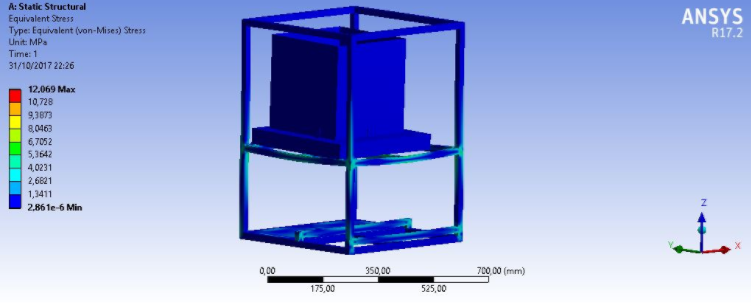
\includegraphics[]{figuras/tensaoequivalente.png}
	\caption{Tensão Equivalente de Von Mises}
\end{figure}

\begin{table}[H]
	\centering
	\caption{Resultados para análise estática}
	\label{analiseestatica}
	\begin{tabular}{|c|c|c|}
		\hline
		Peça                   & Material & Máxima Tensão Equivalente {[}MPa{]} \\ \hline
		Estrutura              & Metalon  & 8,000                               \\ \hline
		Compartimento de Carga & Alumínio & 12,069                              \\ \hline
	\end{tabular}
\end{table}

\subsubsection{Simulação de Transferência de Calor }

O principal objetivo do projeto é o transporte seguro de órgãos, dentro das condições necessárias. Portanto, um dos pontos mais importantes é a refrigeração do órgão para que este esteja sempre em um ambiente com temperatura dentro dos limites aceitáveis.

É interessante portanto, simular a transferência de calor principalmente no compartimento de carga e na câmara de resfriamento. Para isto, foi desenhado um modelo simplificado desses componentes da estrutura em CAD e foi feita uma simulação em ANSYS Steady Thermal.

O modelo utilizado para a simulação é composto de um cubo representando o compartimento de carga e uma caixa representando a câmara de resfriamento, dentro da qual está a serpentina do sistema de refrigeração.

\paragraph*{Condições de contorno}\

\begin{itemize}
	\item Temperatura inicial do compartimento de carga: 2 \textdegree C.
	\item Temperatura inicial da câmara de resfriamento: 0 \textdegree C.
	\item Temperatura dos ambientes de convecção: 0 \textdegree C.
	\item Temperatura na entrada da serpentina: -10 \textdegree C.
	\item Temperatura na saída da serpentina: 0 \textdegree C.
\end{itemize}

A transferência de calor é feita da serpentina para a caixa por convecção com coeficiente de convecção $h = 48,83 W/m^2K$ e da câmara de resfriamento para o compartimento de carga com coeficiente $h = 40 W/m^2K$.

\paragraph*{Resultados}\

\begin{figure}[H]
	\centering
	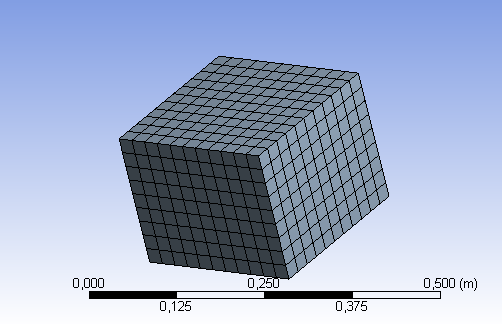
\includegraphics[]{figuras/meshcompartimento.png}
	\caption{Malha do compartimento de carga}
\end{figure}

\begin{figure}[H]
	\centering
	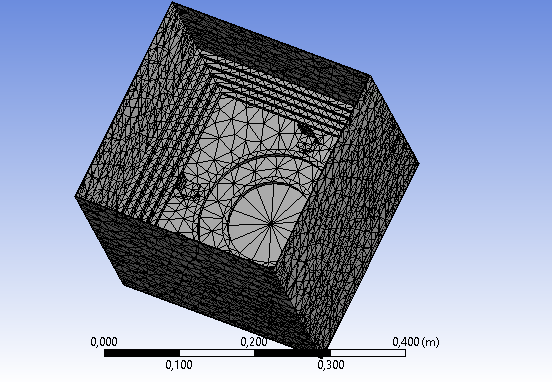
\includegraphics[]{figuras/meshcamara.png}
	\caption{Malha da câmara de resfriamento}
\end{figure}

\begin{figure}[H]
	\centering
	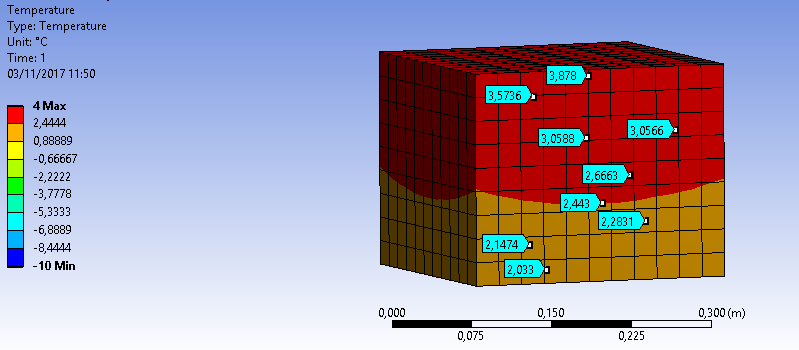
\includegraphics[scale=.7]{figuras/tempcompartimento.png}
	\caption{Distribuição de temperatura no compartimento de carga}
\end{figure}

\begin{figure}[H]
	\centering
	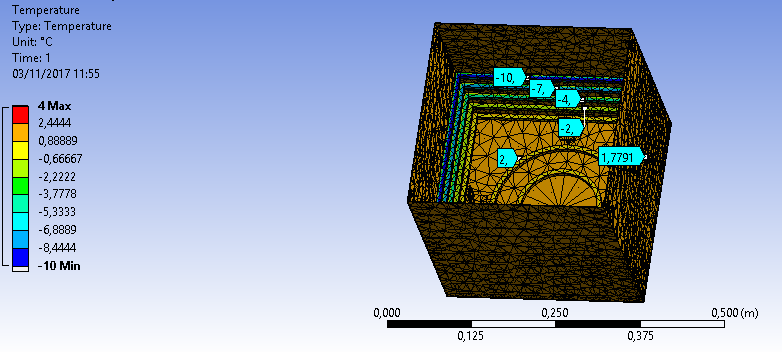
\includegraphics[scale=.7]{figuras/tempcamara.png}
	\caption{Distribuição de temperatura na câmara de resfriamento}
\end{figure}

\begin{figure}[H]
	\centering
	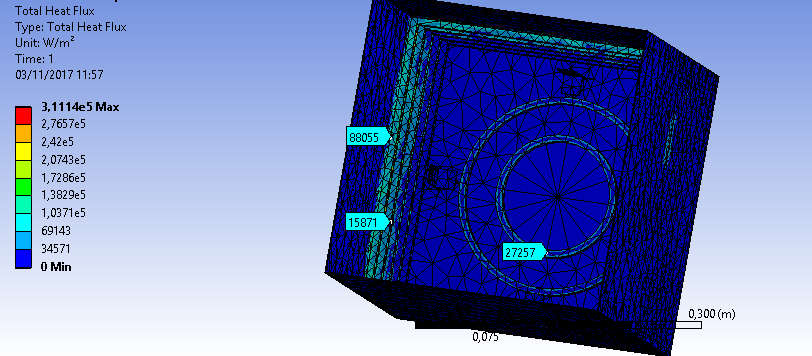
\includegraphics[scale=.7]{figuras/fluxocamara.png}
	\caption{Fluxo de calor na câmara de resfriamento}
\end{figure}

\chapter{Anexos}

\section{Desenhos Técnicos}


\begin{figure}[H]
	\centering
	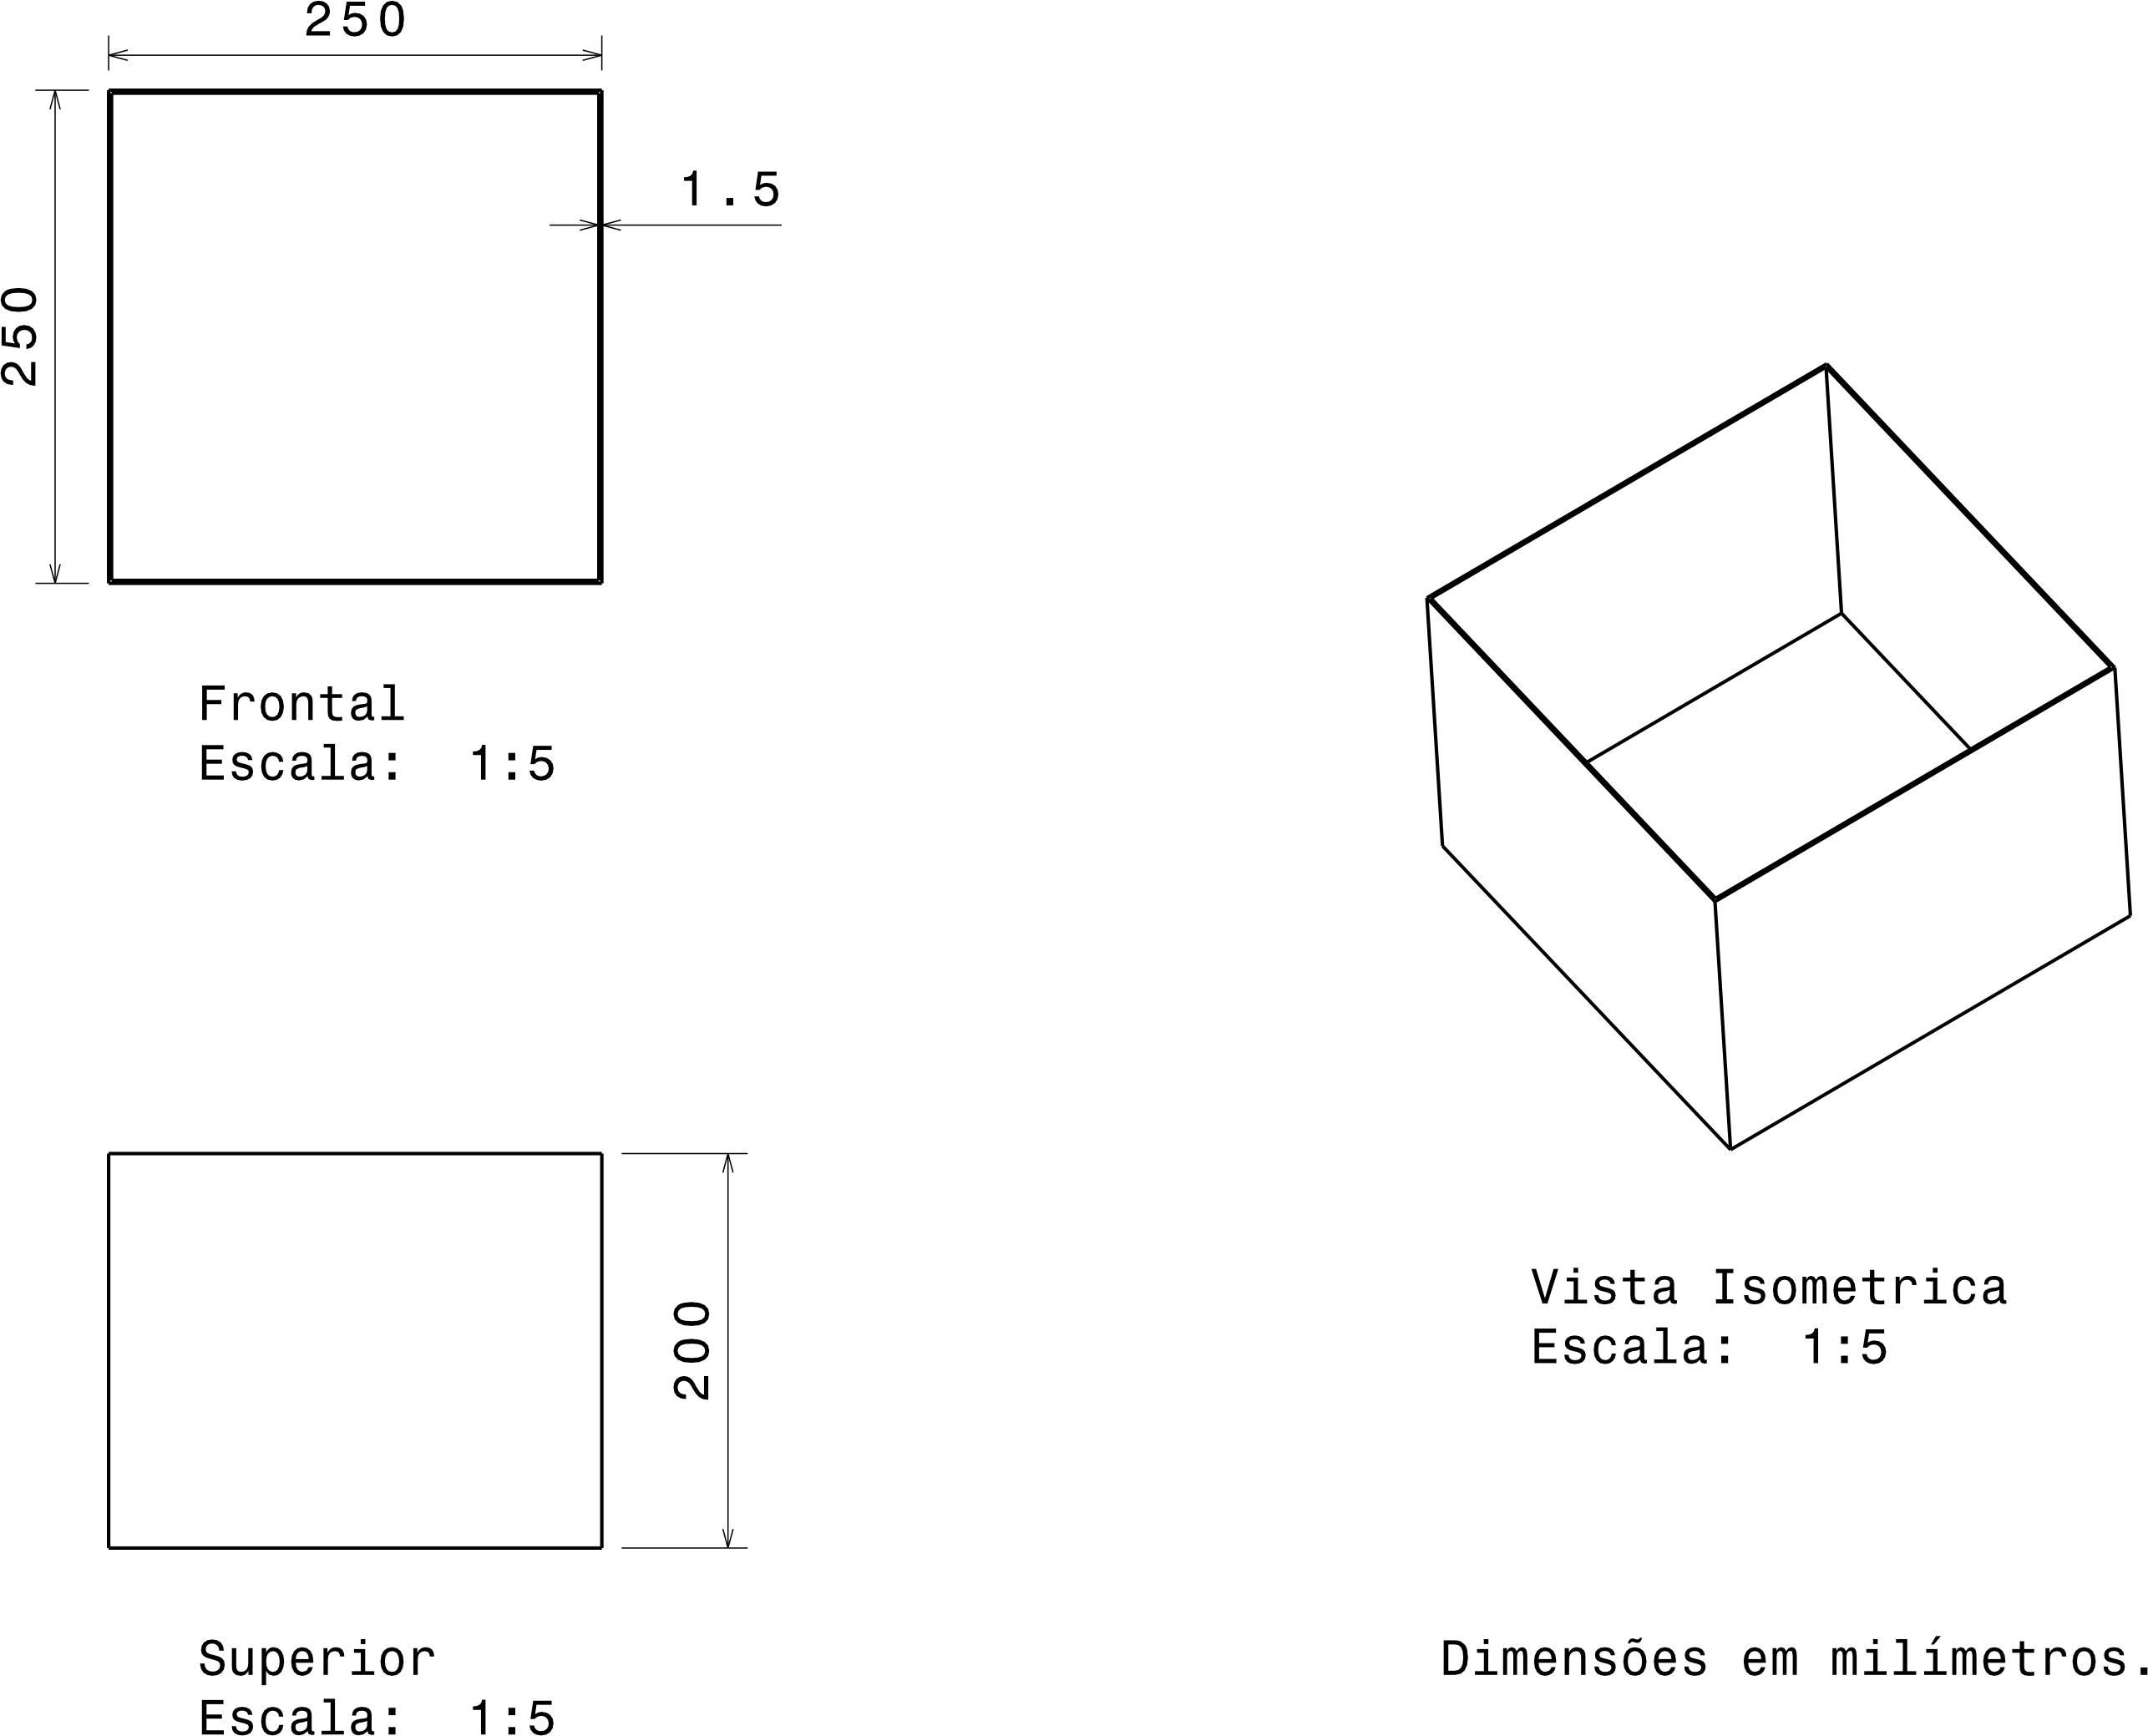
\includegraphics[scale=.5]{figuras/desenho_camara_interna.png}
	\caption{Desenho técnico do compartimento de carga}
\end{figure}


\begin{figure}[H]
	\centering
	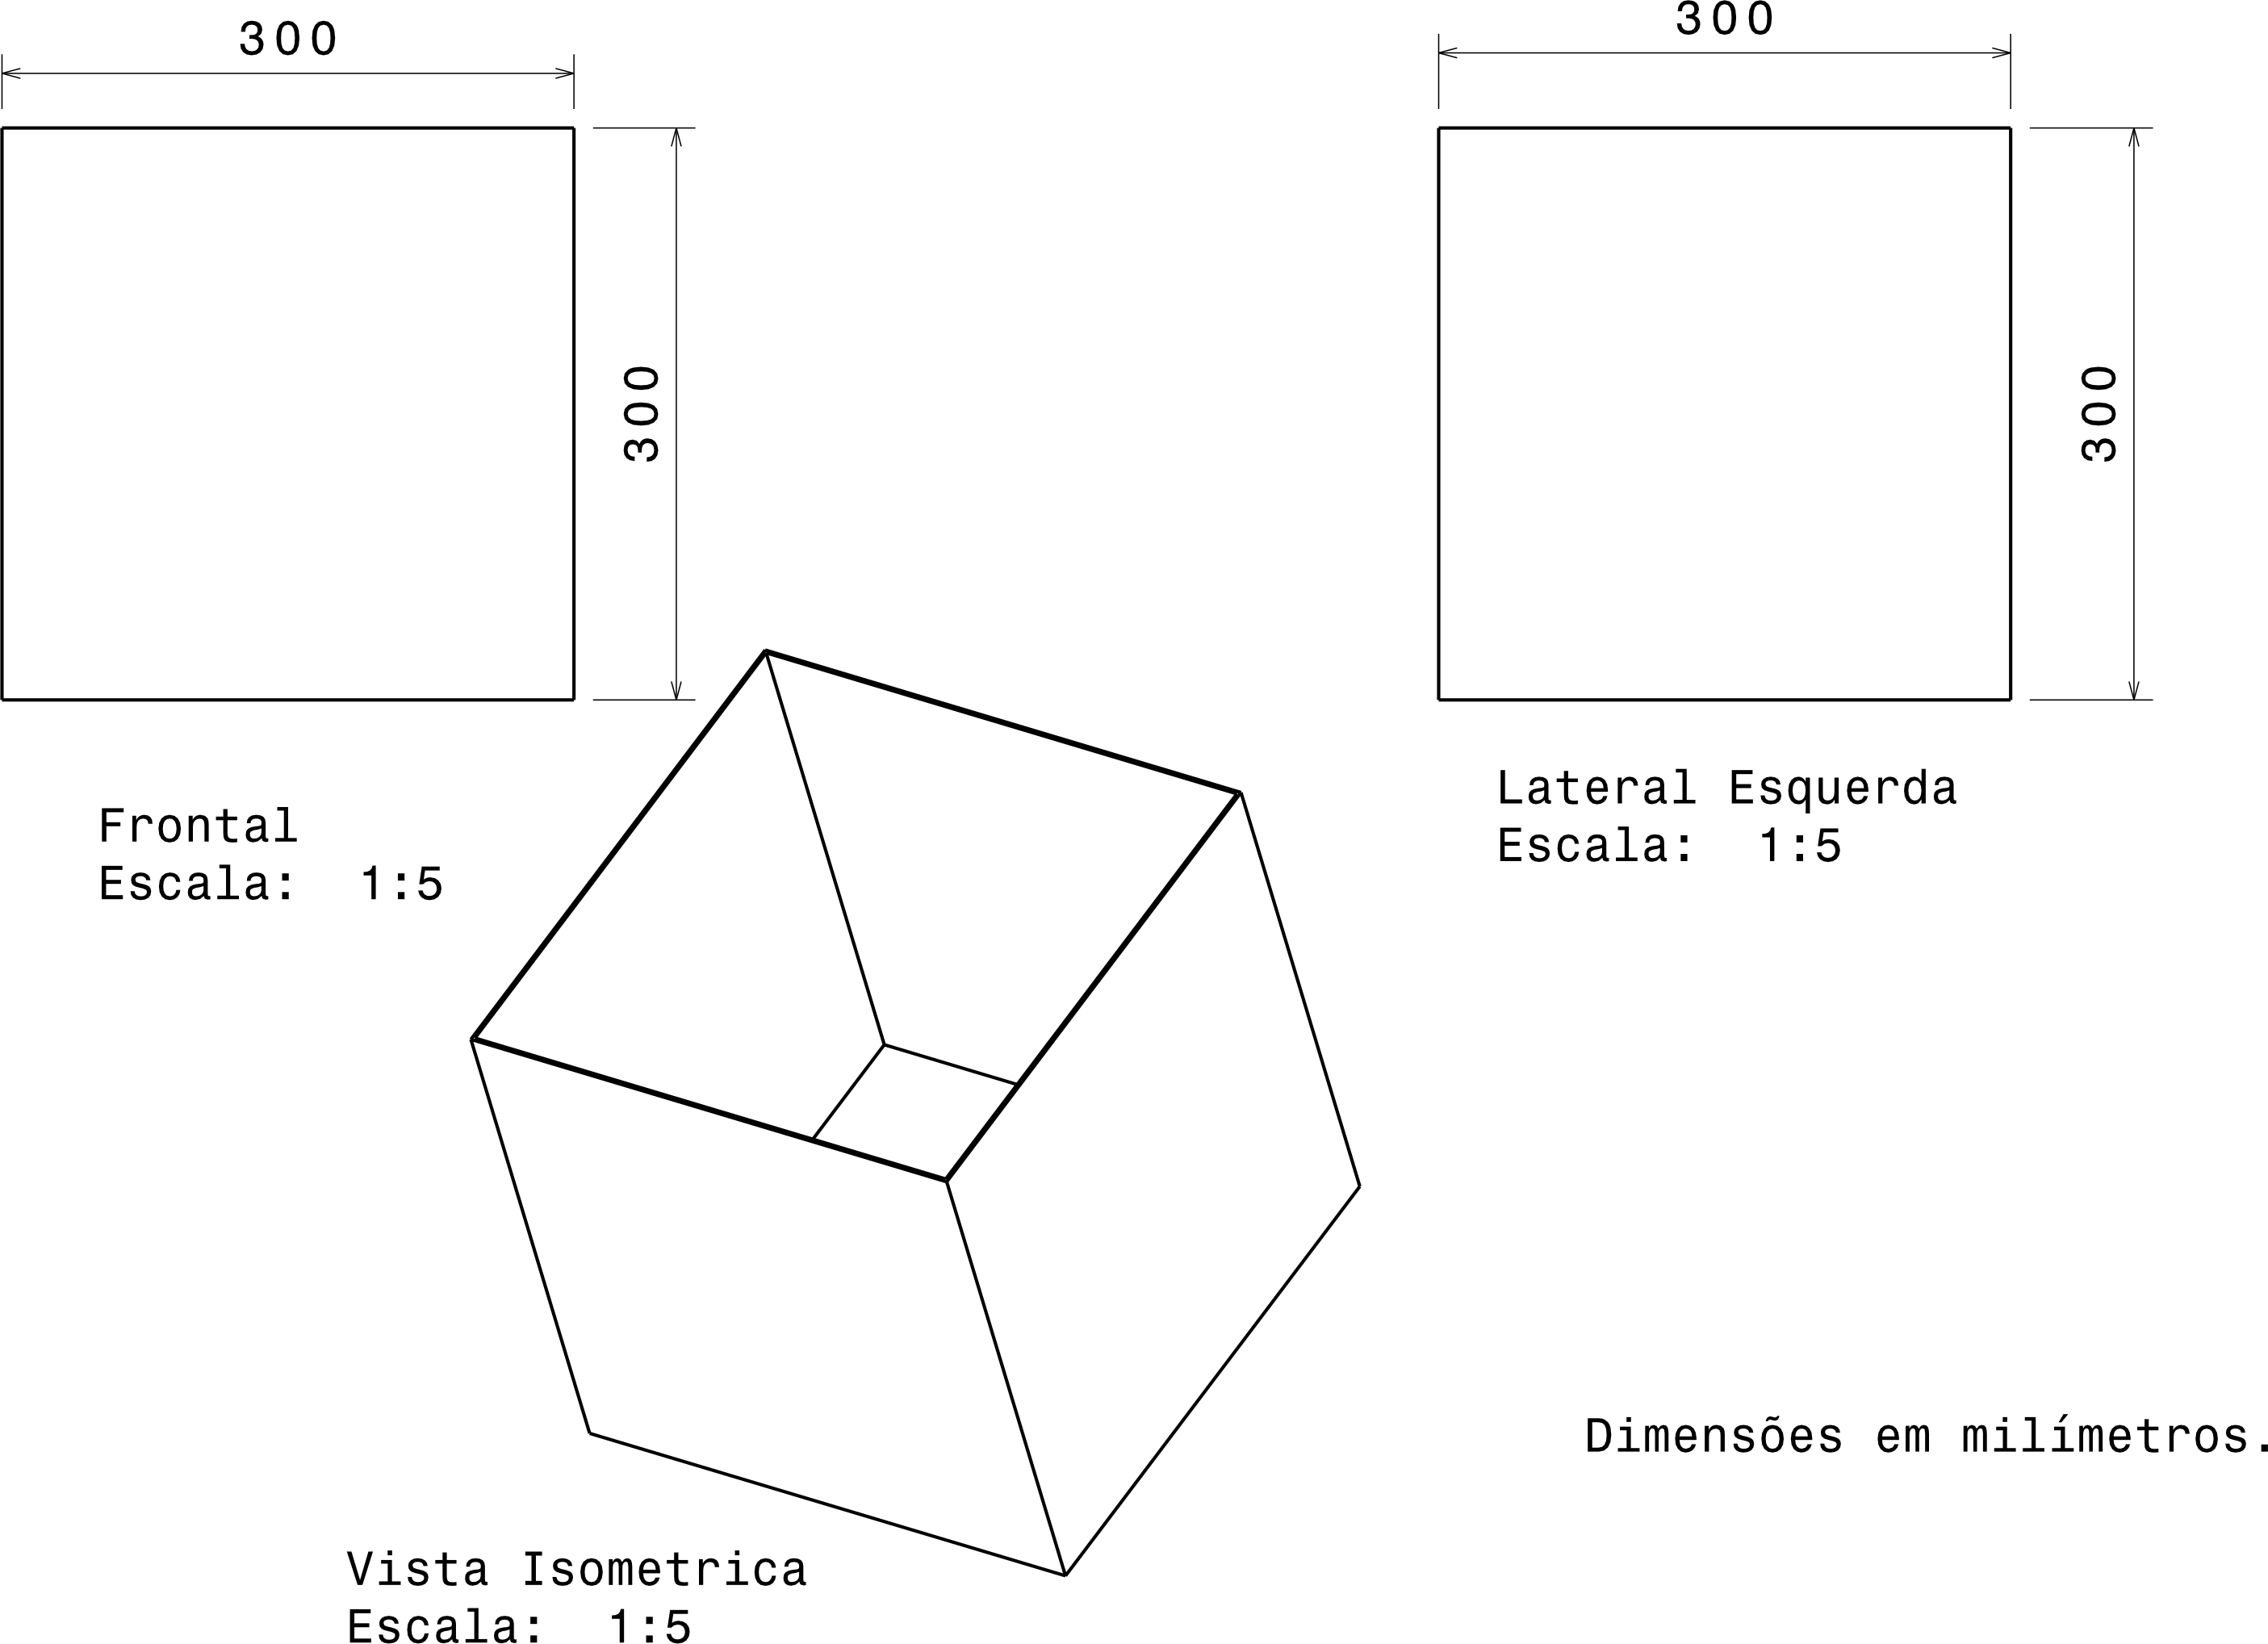
\includegraphics[scale=.5]{figuras/desenho_camara_externa.png}
	\caption{Desenho técnico da câmara de resfriamento}
\end{figure}


\begin{figure}[H]
	\centering
	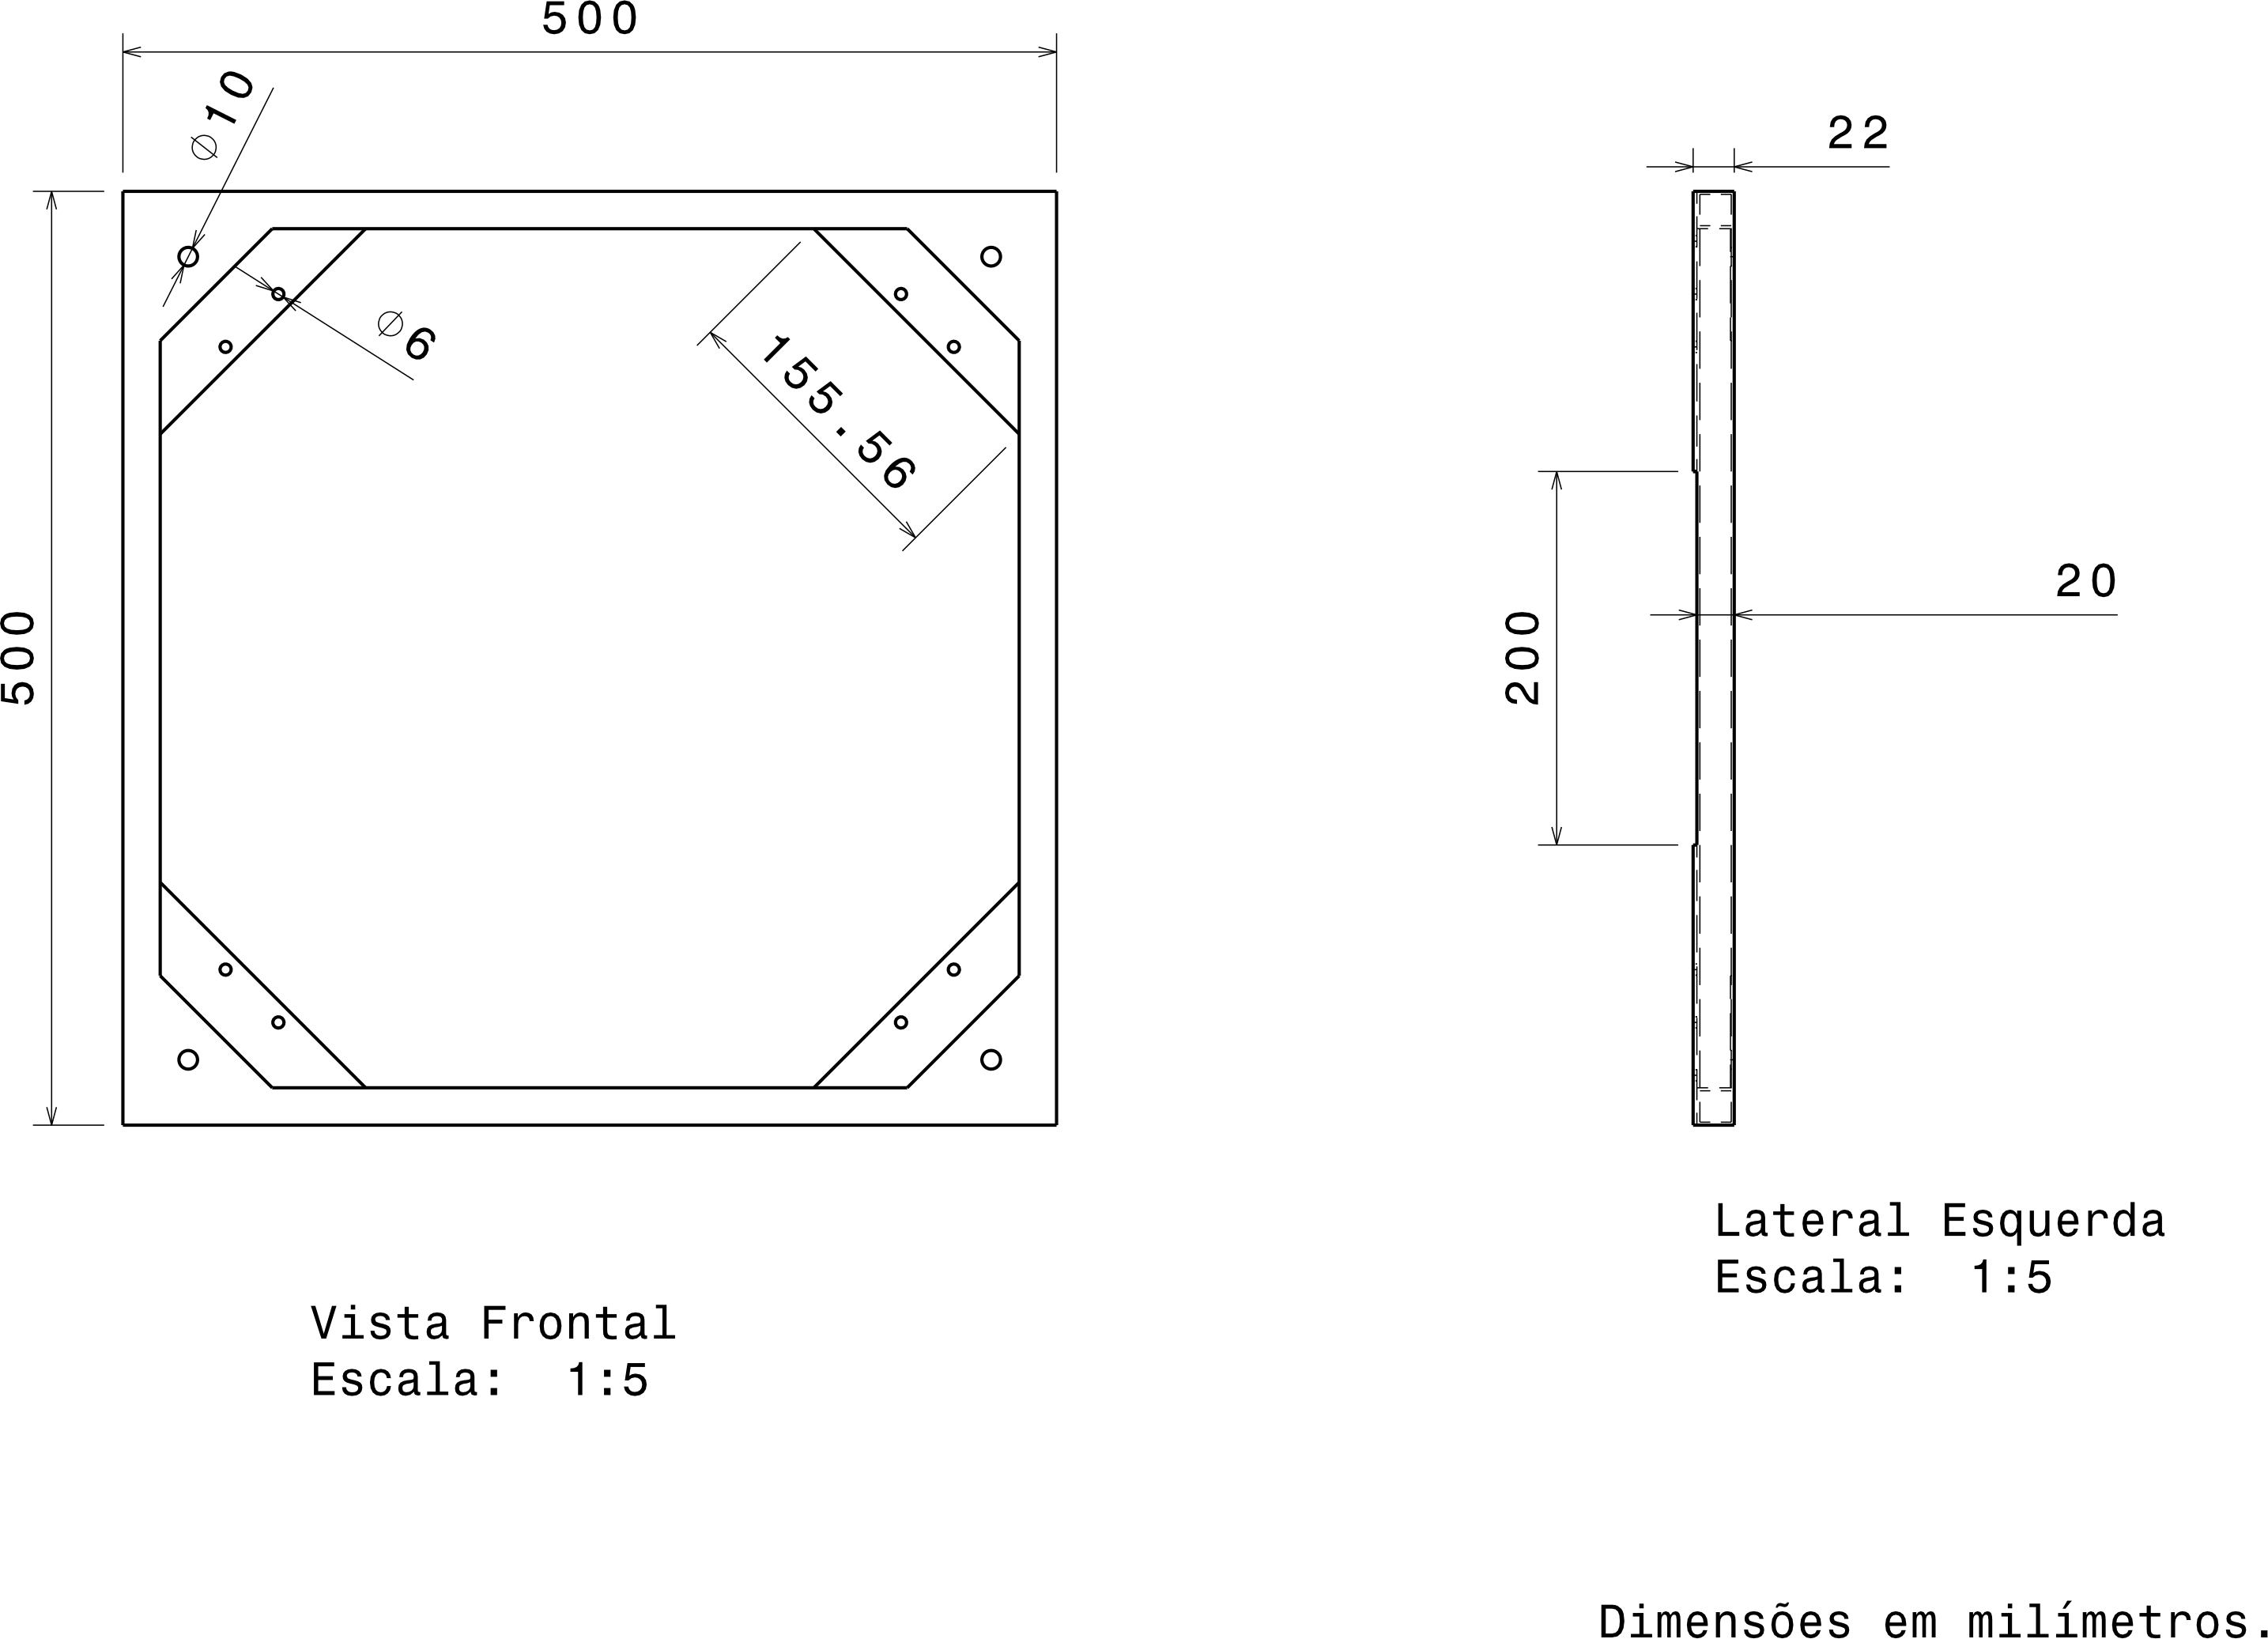
\includegraphics[scale=.5]{figuras/desenho_base.png}
	\caption{Desenho técnico da base da estrutura}
\end{figure}


\begin{figure}[H]
	\centering
	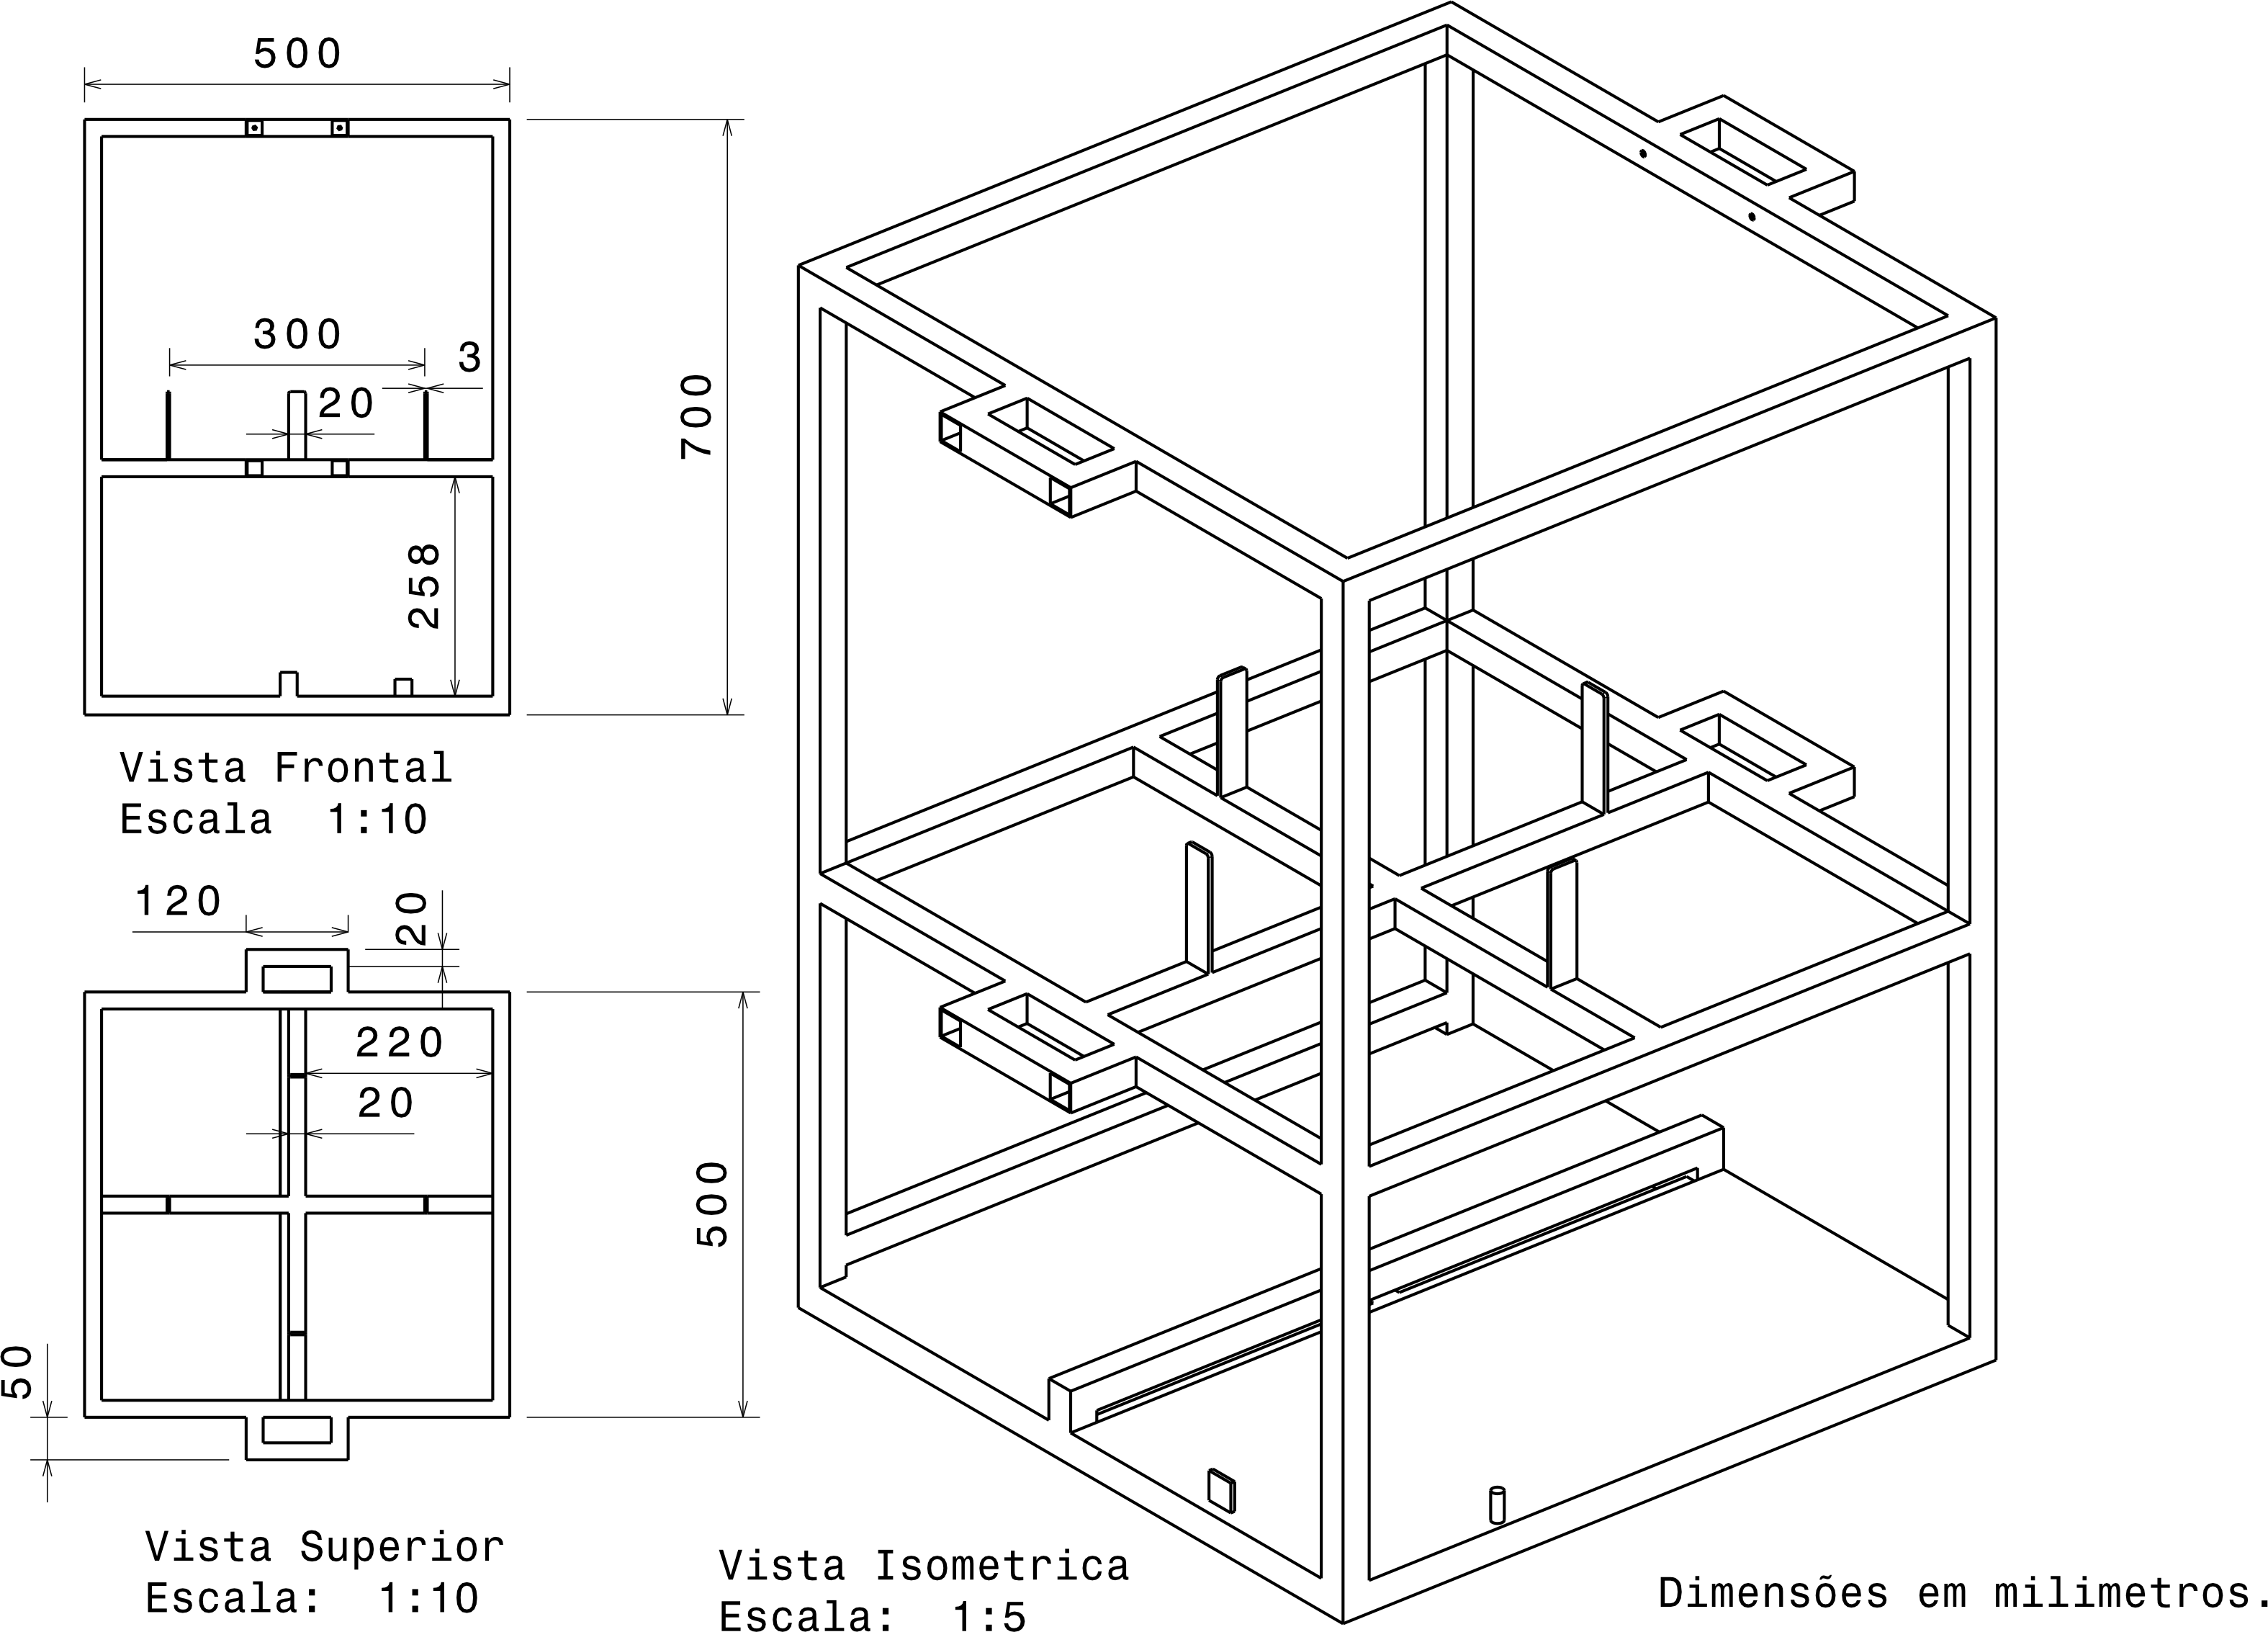
\includegraphics[scale=.5]{figuras/desenho_estrutura.png}
	\caption{Desenho técnico da estrutura principal}
\end{figure}


\begin{figure}[H]
	\centering
	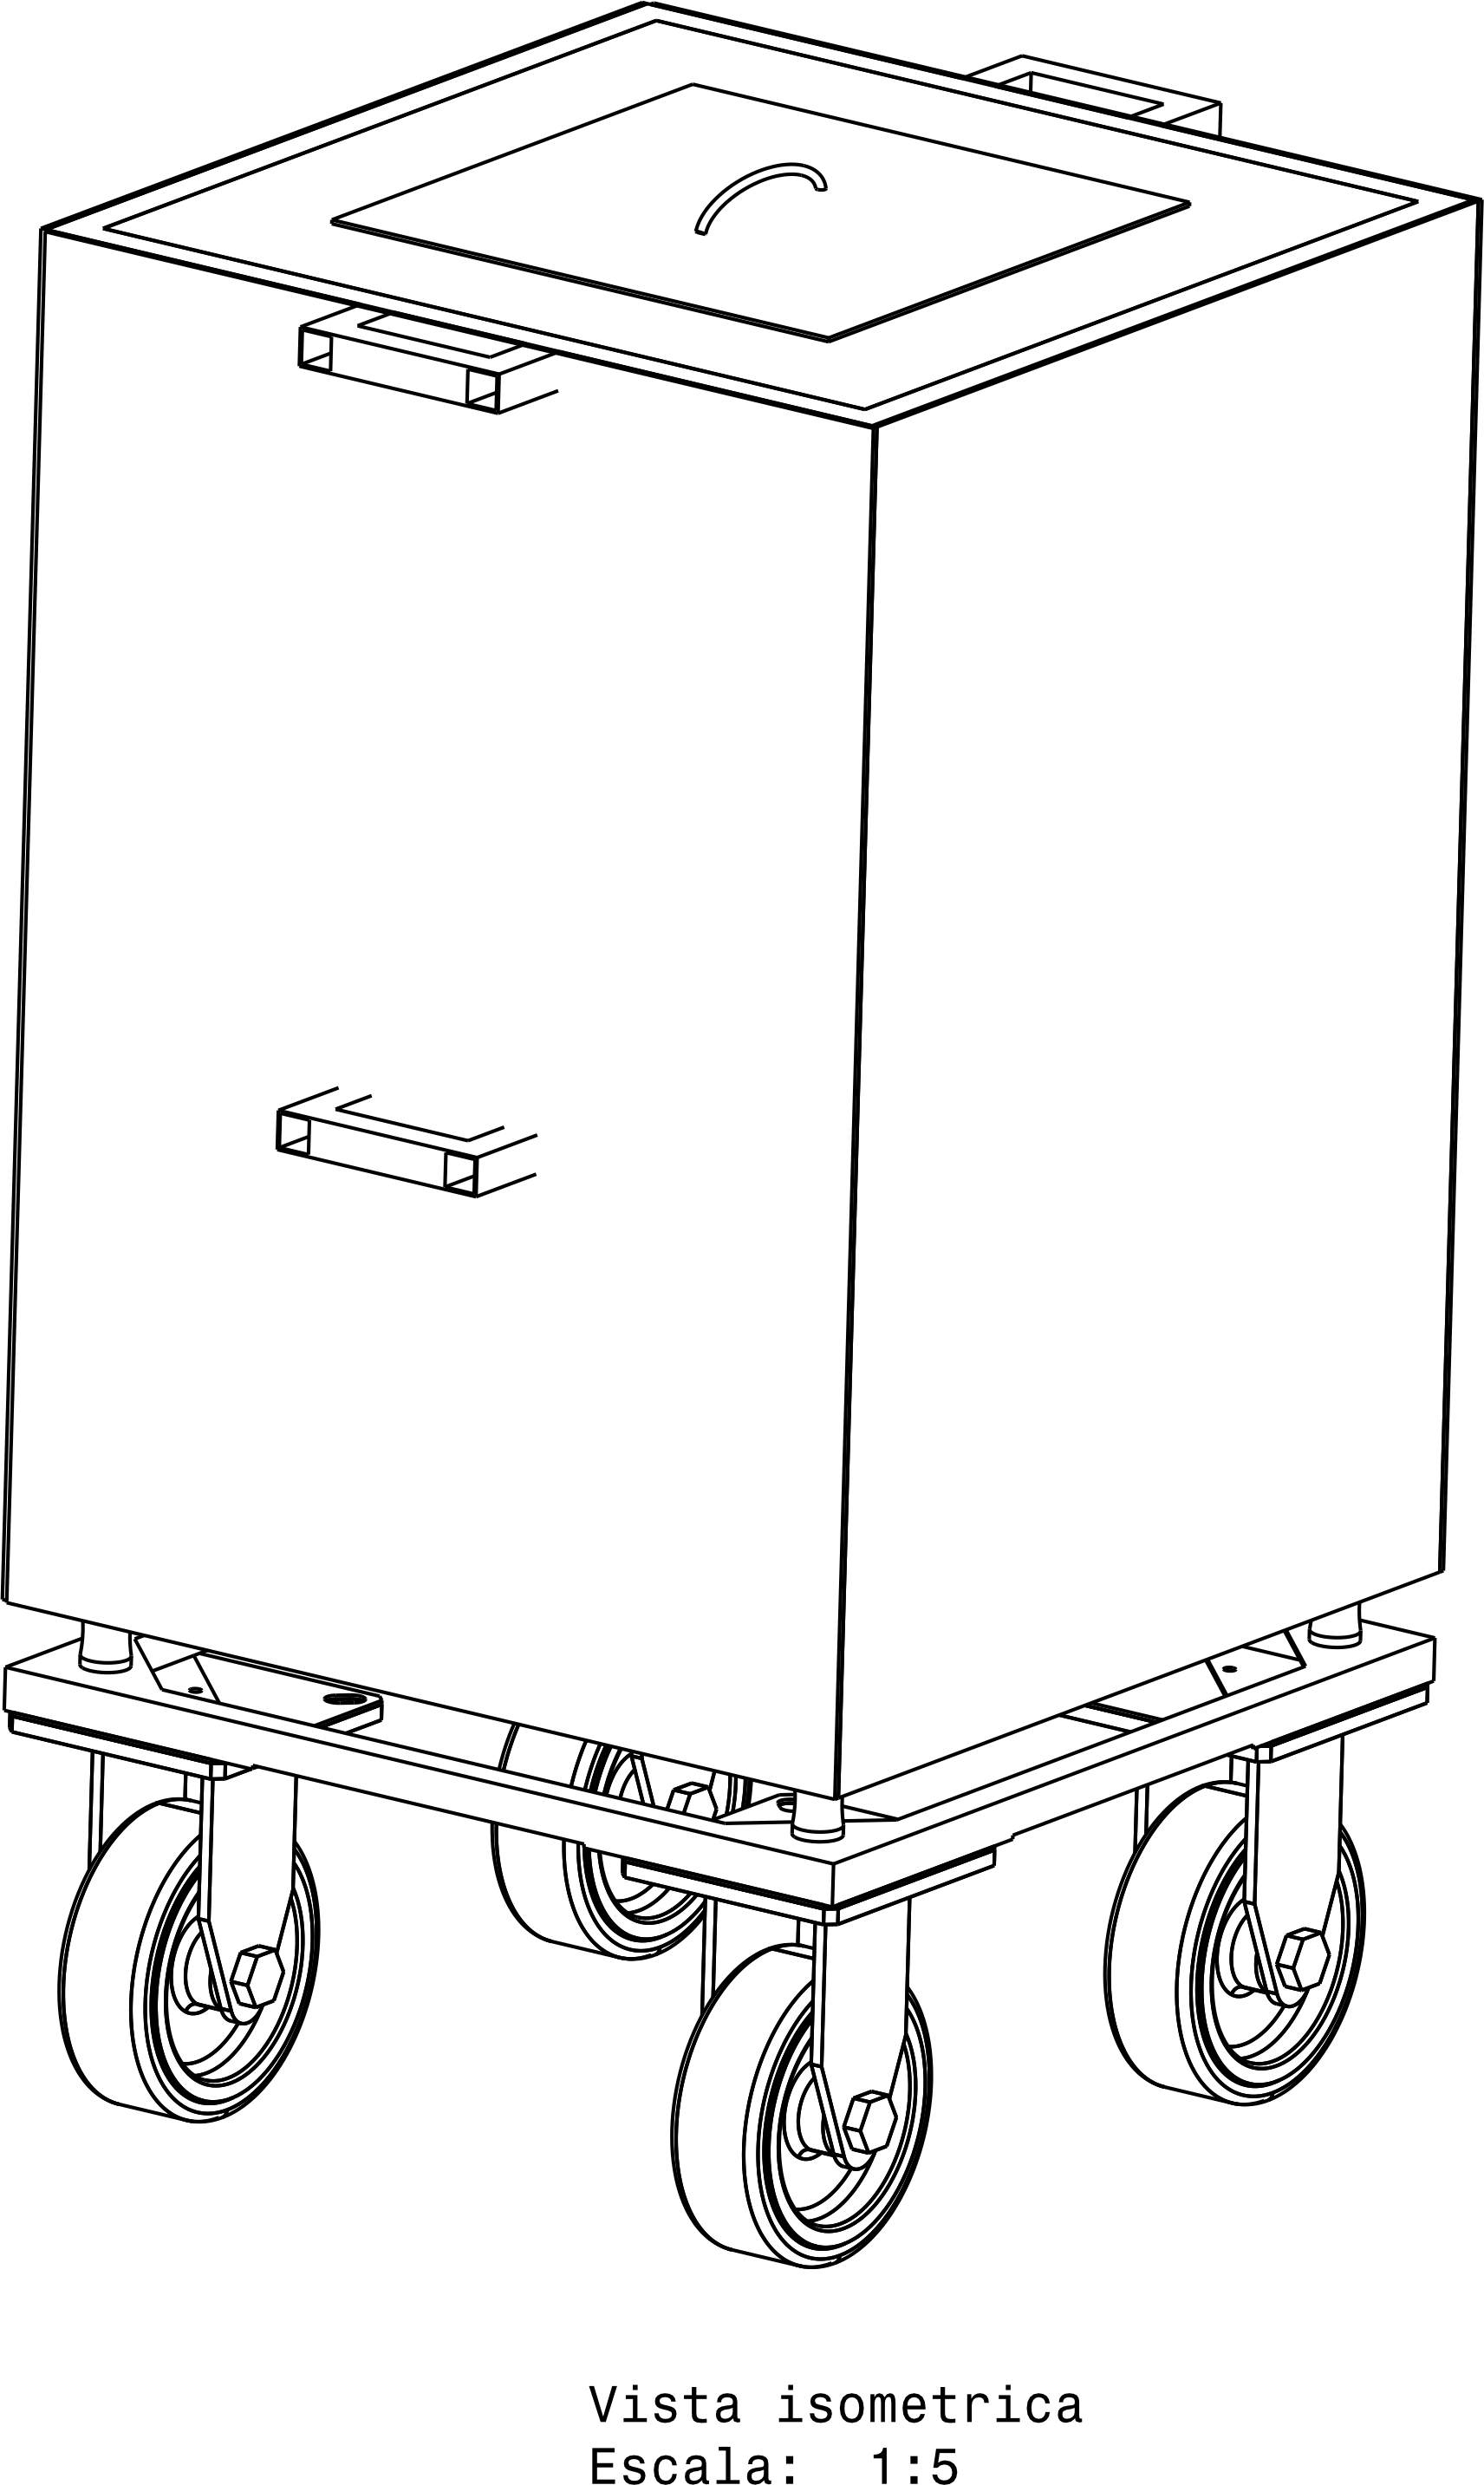
\includegraphics[scale=.5]{figuras/desenho_completo.png}
	\caption{Desenho técnico da estrutura completa}
\end{figure}


\begin{figure}[H]
	\centering
	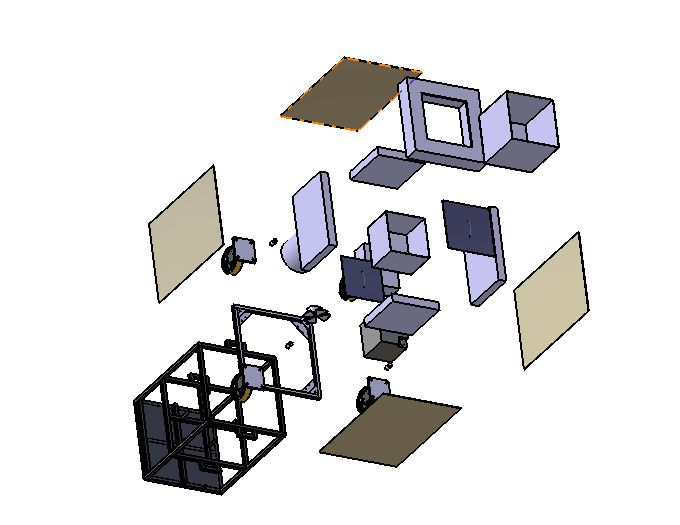
\includegraphics[scale=.5]{figuras/VistaExplodida.jpg}
	\caption{Vista explodida da estrutura}
\end{figure}

\begin{figure}[H]
	\centering
	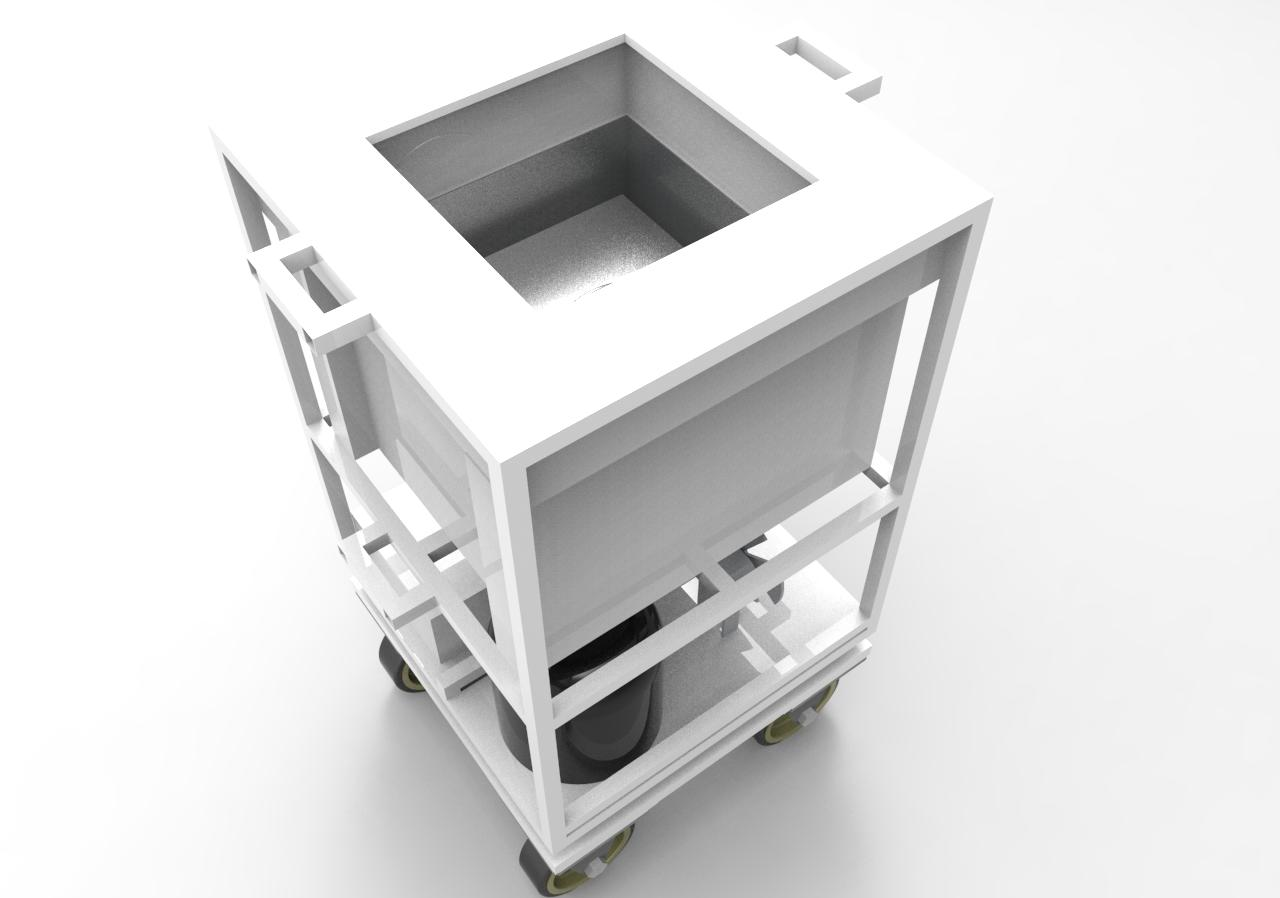
\includegraphics[width=\textwidth]{figuras/render_1.jpg}\
	\includegraphics[scale=.5]{figuras/render_2.jpg}\
	\includegraphics[scale=.5]{figuras/render_3.jpg}
	\caption{Renderizações do desenho técnico}
\end{figure}




